% ------------------------------------------------------------
% ------------------------------------------------------------
  
% Insert the common KETCube AppNote Defines

% ------------------------------------------------------------
% ------------------------------------------------------------

\documentclass[twoside,a4paper,usenames,dvipsnames]{refart}
\usepackage[utf8x]{inputenc}
%\usepackage[czech]{babel}
\usepackage[pdftex]{graphicx}
\graphicspath{{resources/images/}}
\usepackage{caption}% for \captionof
\usepackage{mwe}% contains example-image

% Definition of shortcuts for authornames
%  Sort alphabetically by surname

\newcommand{\JB}{Jan Bělohoubek}
\newcommand{\JC}{Jiří Čengery}
\newcommand{\JF}{Jaroslav Freisleben}
\newcommand{\PK}{Petr Kašpar}
\newcommand{\MU}{Matin Úbl}
\newcommand{\KV}{Kryštof Vaněk}
\newcommand{\JZ}{Jan Záruba}


\usepackage[owncaptions]{vhistory}
\usepackage{hyperref}
%\usepackage[superscript,biblabel]{cite}
\usepackage{multirow}
\usepackage{wrapfig}
\usepackage{float}
\usepackage{siunitx}
\usepackage[table, x11names]{xcolor}
\usepackage{fancyvrb}
\usepackage{fontawesome}
\usepackage[many]{tcolorbox}
\usepackage{listings}
\usepackage{tikz}
\usetikzlibrary{shapes,positioning}
\usepackage{verbatimbox}

\usepackage{array, booktabs, boldline} %
\usepackage{mathtools}
\usepackage[normalem]{ulem}

\usepackage[T1]{fontenc}% Needed for \textquotedbl
\DeclareSIUnit[number-unit-product = {}]{\inchQ}{\textquotedbl}

\newsavebox{\tempbox}
\newlength{\tempheight}

\newcommand\ToDo[1]{\textcolor{red}{ToDo: #1}}

% --- Boxed Enviroments

\newcommand\docNote[1]{
\par
\addvspace{0.5cm}
\subsubsection*{~\hspace{0.2cm}\textcolor{gray}{\Huge \faCommentingO\,}}
\vspace{-1.5cm}
\begin{tcolorbox}[breakable,colback=white,colframe=gray,width=\dimexpr\textwidth+32mm\relax,enlarge left by=-32mm, title = Note]
\it \small #1
\end{tcolorbox}
}

\newcommand\docWarn[1]{
\par
\addvspace{0.5cm}
\subsubsection*{~\hspace{0.2cm}\textcolor{gray}{\Huge \faWarning\,}}
\vspace{-1.5cm}
\begin{tcolorbox}[breakable,colback=white,colframe=gray,width=\dimexpr\textwidth+32mm\relax,enlarge left by=-32mm, title = Warning]
\it #1
\end{tcolorbox}
}

\newcommand\docExample[1]{
\par
\addvspace{0.5cm}
\subsubsection*{~\hspace{0.2cm}\textcolor{gray}{\Huge \faCogs\,}}
\vspace{-1.5cm}
\begin{tcolorbox}[breakable,colback=white,colframe=gray,width=\dimexpr\textwidth+32mm\relax,enlarge left by=-32mm, title = Example]
#1
\end{tcolorbox}
}

\newenvironment{docCodeExample}
{
\par
\addvspace{0.5cm}
\subsubsection*{~\hspace{0.2cm}\textcolor{gray}{\Huge \faCogs\,}}
\vspace{-1.5cm}
\begin{tcolorbox}[breakable,colback=white,colframe=gray,width=\dimexpr\textwidth+32mm\relax,enlarge left by=-32mm, title = Example]
}
{
\end{tcolorbox}
}

\newenvironment{docCodeExampleTitled}[1]
{
\par
\addvspace{0.5cm}
\subsubsection*{~\hspace{0.2cm}\textcolor{gray}{\Huge \faCogs\,}}
\vspace{-1.5cm}
\begin{tcolorbox}[breakable,colback=white,colframe=gray,width=\dimexpr\textwidth+32mm\relax,enlarge left by=-32mm, title = Example: #1]
}
{
\end{tcolorbox}
}

% --- Filesystem Names 
\newcommand\docPath[1]{{\tt #1}}
\newcommand\docFileName[1]{{\tt #1}}

% --- Source Code Names 
\newcommand\docVarName[1]{{\tt #1}}
\newcommand\docFnName[1]{{\tt #1}}
\newcommand\docTypeName[1]{{\tt #1}}

% --- KETCube Terms
\newcommand\docKCModName[1]{{\it #1} module}
\newcommand\docKCCmdInline[1]{\colorbox{gray!30}{\tt #1}}
\newcommand\docKCCmd[1]{{\tt > #1}}

% --- NICE sections
\newcommand\niceSubSection[2]{
\subsection*{~\hspace{0.2cm}{\Huge #1}\\[-0.6cm]\phantom{x}~\hspace{1cm}~#2}
\vspace{-0.7cm}
}

%skryt barevny obdelnik kolem odkazu
\hypersetup{
    colorlinks=false,
    pdfborder={0 0 0},
}

% vhistory
\renewcommand{\vhhistoryname}{Revision History}
\renewcommand{\vhchangename}{Note}
\renewcommand{\vhversionname}{Revision}
\renewcommand{\vhdatename}{Date}
\renewcommand{\vhauthorname}{Author}
\renewcommand \vhAuthorColWidth{0.8\hsize}
\renewcommand \vhChangeColWidth{1.2\hsize}

\DeclareRobustCommand{\UWBLogo}{%
   \begin{wrapfigure}{l}{2.1cm}
    \vspace{-1.35cm}
    \includegraphics[width=2cm]{ZCU_logo.pdf}
   \end{wrapfigure}
}


% declare the path(s) where your graphic files are
% extract presenattion number to create include path for images
\ExplSyntaxOn
% Save a copy of \jobname
\tl_set:NV \NUMBER \c_sys_jobname_str
\regex_replace_once:nnN { [A-Za-z]*_[A-Za-z]*_ } { } \NUMBER
\ExplSyntaxOff

% declare the path(s) where your graphic files are
%\graphicspath{{resources/images/}{resources/appNotes/001/images/}}
\graphicspath{{resources/images/}{resources/appNotes/\NUMBER/images/}}
\graphicspath{{resources/images/}{resources/appNotes/003/images/}}

\pdfinfo
{
  /Title       (The KETCube Project AppNote)
  /Creator     (LaTeX)
  /Author      (The SmartCAMPUS Team)
}




\title{\UWBLogo KETCube AppNote 008:\\ KETCube Bootloader (\vhCurrentVersion)}

\author{Author: \vhListAllAuthorsLongWithAbbrev}
\date{Version \vhCurrentVersion\ from \vhCurrentDate}

% ------------------------------------------------------------
% ------------------------------------------------------------
  
% Insert the common KETCube AppNote Head

% ------------------------------------------------------------
% ------------------------------------------------------------

\begin{document}
\pagenumbering{roman} 

\titlepage
\maketitle

% ------------------------------------------------------------
% ------------------------------------------------------------
  
% BEGIN of the KETCube appNote Content

% ------------------------------------------------------------
% ------------------------------------------------------------


% ------------------------------------------------------------
% ------------------------------------------------------------
  
% BEGIN of the KETCube appNote Content

% ------------------------------------------------------------
% ------------------------------------------------------------

\section*{KETCube Bootloader: the STM Bootloader Re-Invented}
{\it KETCube} \cite{ZCU:KETCube:05-2018} is the prototyping and demo platform developed at the Department of Materials and Technology (KET), University of West Bohemia in Pilsen. 


This document describes the KETCube Bootloader. The bootloader is in part compatible with the standard ROM STM32 bootloader \cite{STM32:AN3155}. It was designed to provide a basic bootloader for the KETCube platform compatible with the standard toolset but equipped employed by customizable parameters, such as command timeouts.

\setcounter{tocdepth}{2}
\tableofcontents
\clearpage

\listoffigures
\listoftables
\begin{versionhistory}
  \vhEntry{0.2.0*}{8.6.2021}{JB}{Initial version}
\end{versionhistory}
% history table ... do not number
\setcounter{table}{0}

\clearpage 
\pagenumbering{arabic} 
\pagestyle{headings} 

\clearpage
\section{Bootloader Architecture} \label{sec:arch}

\marginlabel{\captionof{figure}{Bootloader operation sequence}\label{fig:bootOp:sequence}}
\raisebox{-\height}{\scalebox{0.7}{\begin{tikzpicture}[font=\small,thick]
 
\node[draw,
    rounded rectangle,
    minimum width=3.5cm,
    minimum height=1cm,
    align=center
] (block0) { Start Bootloader };
 
\node[draw,
    diamond,
    below=of block0,
    minimum width=3.5cm,
    minimum height=1cm,
    align=center
] (block1) { 0x7F or command received\\in the time window\footnotemark\\on supported interface };

\node[draw,
    below=of block1,
    minimum width=3cm,
    minimum height=1cm,
    align=center
] (block2) { USART1 selected };

\node[draw,
    below=of block2,
    minimum width=3cm,
    minimum height=3cm,
    align=center
] (block3) { Auto-baud rate sequence\\send ACK byte \& disable\\unused peripherals\footnotemark };

\node[coordinate,below=1cm of block3] (blockCmdWait) {};

\node[draw,
    diamond,
    below=1cm of blockCmdWait,
    minimum width=3cm,
    minimum height=2cm,
    align=center
] (block4) { Wait for a\\command };
 
\node[coordinate,below=1cm of block4] (blockCmdRecv) {};

\node[draw,
    below=of blockCmdRecv,
    minimum width=3cm,
    minimum height=2cm,
    align=center
] (block6) { Basic Commands\\(Get, Read, Write, \dots) };

\node[draw,
    right=of block6,
    minimum width=3cm,
    minimum height=2cm,
    align=center
] (block7) { GO cmd\\routine };

\node[below=1cm of block7, fill=white] (blockJumpAddr) {Jump To Address};
\node[right=of blockJumpAddr, fill=white] (blockJumpApp) {Jump To Application};

\node[coordinate,below=1cm of block6] (blockCmdExec) {};
\node[coordinate,below=1cm of blockCmdExec] (blockCmdExec2) {};
\node[coordinate,left=5cm of blockCmdExec2] (blockCmdExec3) {};
 
% Arrows
\draw[-latex] (block0) edge (block1)
              (block2) edge (block3)
              (block3) -- (blockCmdWait)
              (blockCmdWait) -| (block4)
              (block4) edge (blockCmdRecv);
              
\draw[->] (block1) -- (block2) node [pos=0.5,right,font=\footnotesize] { Yes };
\draw[->] (block1) -| (blockJumpApp) node [pos=0.1,above,font=\footnotesize] { No };
              
\draw[->] (blockCmdRecv) -| (block6);
\draw[->] (blockCmdRecv) -| (block7);

\draw[] (block6) |- (blockCmdExec);
\draw[->] (block7) -- (blockJumpAddr);

\draw[] (blockCmdExec) |- (blockCmdExec2)
        (blockCmdExec2) |- (blockCmdExec3);
\draw[->] (blockCmdExec3) |- (blockCmdWait);
 
\end{tikzpicture}}}
\addtocounter{footnote}{-1}
\footnotetext{The dafault time window for 0x7F reception is 5 seconds}
\addtocounter{footnote}{+1}
\footnotetext{Autobaudrate is currently NOT supported by this bootloader}

\subsection{Bootloader Configuration}
  The primary clock source is MSI at 2.097 MHz.
  
  Independent watchdog (IWDG) is currently not handled by the bootloader -- currently, it might cause problems if previously enabled by the application.

\subsection{Interfaces}

\subsubsection{UART1 Settings}

\begin{itemize}
  \item Tx PIN: PA9
  \item Rx PIN: PA10
  \item Default Baud Rate: 57600 bps
  \item Data bits: 8
  \item Stop bits: 1
  \item Parity: Even
  \item HW Flow control: No
\end{itemize}

\subsubsection{Auto-Baud Rate}
\docNote{The auto-baud rate is currently not implemented.}

\subsection{Memory Map} \label{sec:arch:map}

\marginlabel{\captionof{figure}{Program Flash}\label{fig:cmd:get}}
\raisebox{-\height}{

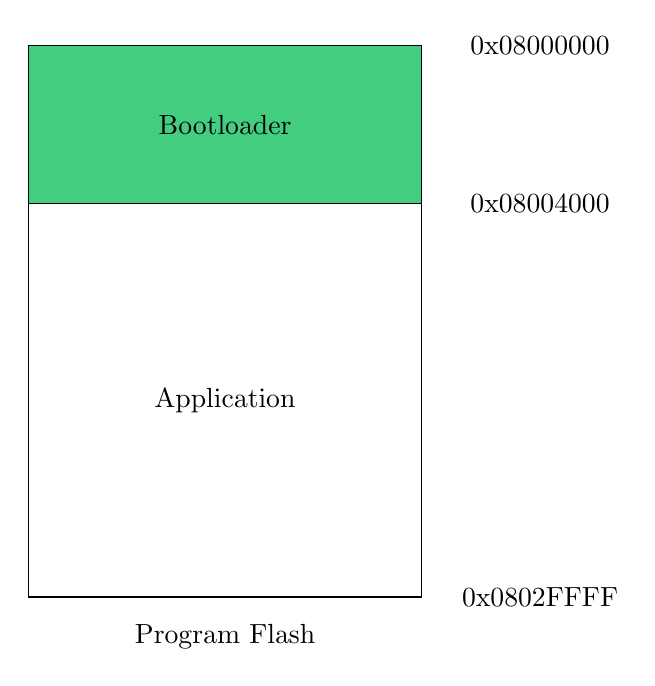
\begin{tikzpicture}
  \node[draw,fill=white,    minimum height=5cm,minimum width = 5cm,yshift=0cm](10/5){Application};
  \node[draw,fill=SeaGreen3,minimum height=2cm,minimum width = 5cm,yshift=3.5cm](10/5){Bootloader};
  
  \node[anchor=center,yshift=4.5cm,xshift=4cm,fill=white] {0x08000000};
  \node[anchor=center,yshift=2.5cm,xshift=4cm,fill=white] {0x08004000};
  \node[anchor=center,yshift=-2.5cm,xshift=4cm,fill=white] {0x0802FFFF};
  
  \node[anchor=center,yshift=-3.0cm,xshift=0cm,fill=white] {Program Flash};
\end{tikzpicture}
}

\marginlabel{\captionof{figure}{Non-Volatile Data Memory (EEPROM)}\label{fig:cmd:get}}
\raisebox{-\height}{

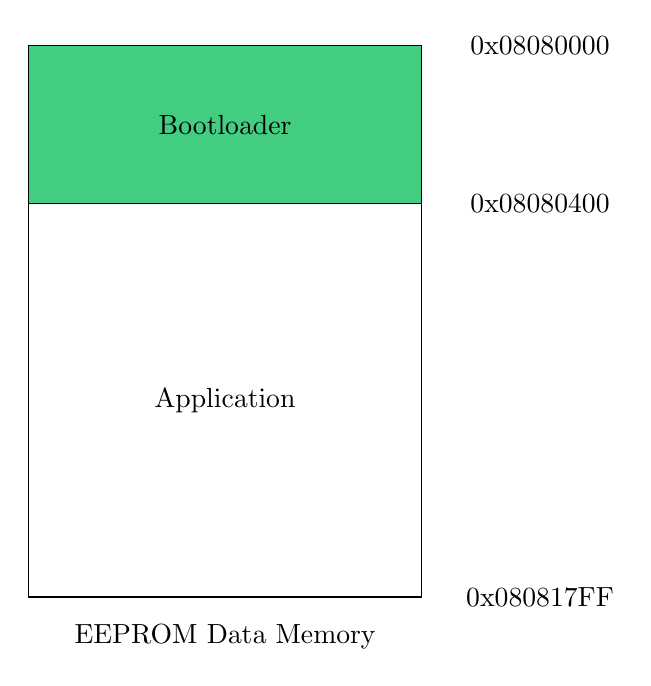
\begin{tikzpicture}
  \node[draw,fill=white,    minimum height=5cm,minimum width = 5cm,yshift=0cm](10/5){Application};
  \node[draw,fill=SeaGreen3,minimum height=2cm,minimum width = 5cm,yshift=3.5cm](10/5){Bootloader};
  
  \node[anchor=center,yshift=4.5cm,xshift=4cm,fill=white]  {0x08080000};
  \node[anchor=center,yshift=2.5cm,xshift=4cm,fill=white]  {0x08080400};
  \node[anchor=center,yshift=-2.5cm,xshift=4cm,fill=white] {0x080817FF};
  
  \node[anchor=center,yshift=-3.0cm,xshift=0cm,fill=white] {EEPROM Data Memory};
\end{tikzpicture}
}

\marginlabel{\captionof{figure}{Volatile Memory (RAM)}\label{fig:cmd:get}}
\raisebox{-\height}{

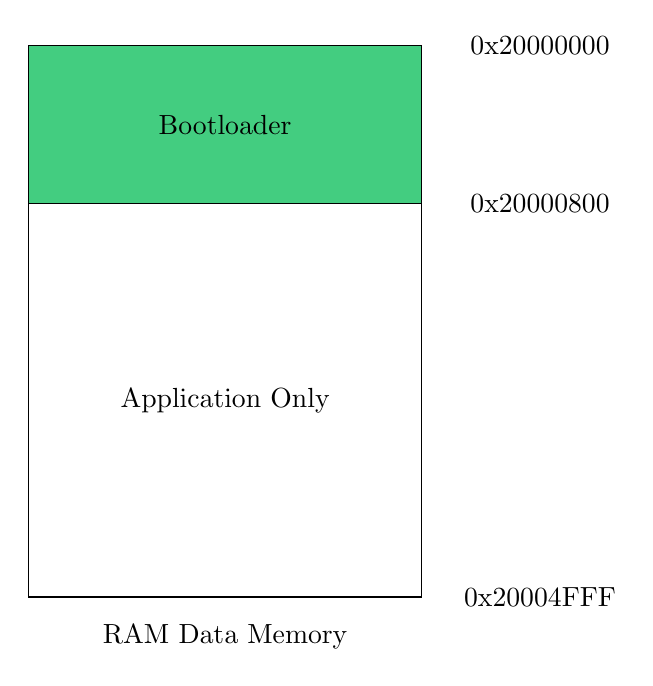
\begin{tikzpicture}
  \node[draw,fill=white,    minimum height=5cm,minimum width = 5cm,yshift=0cm](10/5){Application Only};
  \node[draw,fill=SeaGreen3,minimum height=2cm,minimum width = 5cm,yshift=3.5cm](10/5){Bootloader};
  
  \node[anchor=center,yshift=4.5cm,xshift=4cm,fill=white]  {0x20000000};
  \node[anchor=center,yshift=2.5cm,xshift=4cm,fill=white]  {0x20000800};
  \node[anchor=center,yshift=-2.5cm,xshift=4cm,fill=white] {0x20004FFF};
  
  \node[anchor=center,yshift=-3.0cm,xshift=0cm,fill=white] {RAM Data Memory};
\end{tikzpicture}
}

\docNote{RAM used by the bootloader cannot be re-used by Application!}

\docNote{Structure of pointers to Bootloader API is provided at the gbeginnig of the RAM area.}

\clearpage
\subsection{Non-Volatile Bootloader Configuration} \label{sec:arch:nvm}

\docNote{Application can use the bootloader API to set-up the bootloader. Alternativelly, application can write to the bootloader Non-Volatile Configuration memory to affect future bootloader behaviour -- e.g. appliaction can be used to manage bootloader keys.}

\begin{table*}[!ht]
  \hspace*{-4cm}
  \begin{tabular}{| p{4cm} | p{9cm} | }
      \hline
      \rowcolor{SeaGreen3!30!} {\bf Type} & {\bf Description} \\
      \hline
      \hline
      {\tt startup\_t }  & {\tt 0x00} -- start application code immediatelly (do not enter bootloader);\newline
                          {\tt 0x01} -- stay in bootloader until timeout;\newline 
                          {\tt 0x02} -- stay in bootloader until go\\
      \hline
      {\tt security\_t } & {\tt 0x00} -- do not verify application code;\newline
                           {\tt 0x01} -- check application code CMAC;\newline 
                           {\tt 0x02} -- decrypt application code;\newline
                           {\tt 0x03} -- decrypt application code and check CMAC\\
      \hline
      {\tt uint32\_t}    & Application Startup Timeout in milliseconds \\
      \hline
      {\tt uint32\_t *}  & Application Code start address;\newline
                         do not jump to application if {\tt NULL} \\
      \hline
      {\tt uint8\_t[16]} & Bootloader Unlock Key (bootloader is unlocked if {\tt NULL}) \\
      \hline
      {\tt uint8\_t[16]} & CMAC Key \\
      \hline
      {\tt uint8\_t[16]} & Encryption Key \\
      \hline
  \end{tabular}
  \addcontentsline{lot}{table}{Bootloader Configuration Structure}
  \label{tab:cfgStruct}
 \end{table*}

 
\clearpage
\subsection{Bootloader API} \label{sec:arch:api}
\subsubsection*{Set-Up Bootloader}

\subsubsection*{AES}


\clearpage
\subsection{Application Requirements}
\subsubsection*{Application must}
\begin{itemize}
  \item respect the memory map defined by the bootloader
\end{itemize}

\subsubsection*{Application should not}
\begin{itemize}
  \item modify \docVarName{VTOR}\footnote{\docVarName{Vector Table Offset Register} -- defines the offset of the interrupt vector table in the ARM memory} register -- e.g. applications generated by STM32Cube set the \docVarName{VTOR} register to the beginnig of the flash area
\end{itemize}

\subsubsection*{Prior executing the application code,\\the bootloader sets}
\begin{itemize}
  \item the application stack to the value stored at the first word of the application flash area
  \item the interrupt vector to the beginning of the application area
\end{itemize}

\clearpage
\section{Supported Devices}\label{sec:supportedDevices}

\docNote{This bootloader is designed to be generic, however, it is currently tested only on STM32L0[7,8][1-3] devices.}

\subsection{Adding a New Device}

To add a new device, insert the device definitions to the \docFileName{device.h} file, create the custom memory map in the \docFileName{memory} directory and include it to the linker script  \docFileName{LinkerScript.ld}. For the STM32 devices specification details, see Table 149 in \cite{STM32:AN2606}.

Always use the macro conditional expression to add a new device, e.g. \docVarName{\#if defined(STM32L071xx)}.

\docNote{To select the device, set \docVarName{DEVICE} variable in the Makefile to the device-speciffic string, e.g. to \docVarName{STM32L071xx} to select STM32l071 device.}


\clearpage
\section{Testing}

\subsection{Default Flash Tool}

The primary tool intended for use in connection with this bootloader is {\it stm32flash\footnote{\url{https://sourceforge.net/projects/stm32flash/}}}.

\begin{docCodeExampleTitled}{Test Bootloader Connection}
\begin{verbatim}
$ ./stm32flash -c /dev/ttyUSB0 
stm32flash 0.5_KETCube

http://stm32flash.sourceforge.net/

Interface serial_posix: 57600 8E1
Version      : 0x01
Option 1     : 0x00
Option 2     : 0x00
Device ID    : 0x0447 (STM32L07xxx/08xxx)
- RAM        : Up to 20KiB  (8192b reserved by bootloader)
- Flash      : Up to 192KiB (size first sector: 32x128)
- Option RAM : 32b
- System RAM : 8KiB
\end{verbatim}
\end{docCodeExampleTitled}

\subsection{Test Set}

\begin{docCodeExampleTitled}{Regression Tests}
\begin{verbatim}
$ bash run_tests.sh
...

$ All test cases PASSED!
\end{verbatim}
\end{docCodeExampleTitled}

\clearpage
\section{Boootloader Command Set}

  \begin{table*}[!ht]
    \hspace*{-4cm}
    \begin{tabular}{| p{4cm} | p{1.5cm} | p{7.5cm} |}
        \hline
        \rowcolor{SeaGreen3!30!} {\bf Command} & {\bf CMD Code} & {\bf Description} \\
        \hline
        \hline
        \nameref{cmd:get} & 0x00 & Get bootloader version and the list of commands supported by bootloader \\
        \hline
        \nameref{cmd:getVersion} & 0x01 & Get bootloader version \\
        \hline
        \nameref{cmd:getID} & 0x02 & Get the Chip ID \\
        \hline
        \nameref{cmd:readMem} & 0x11 & Read Memory \\
        \hline
        \nameref{cmd:go} & 0x21 & Go \\
        \hline
        \nameref{cmd:writeMem} & 0x31 & Write Memory \\
        \hline
        \nameref{cmd:extEraseMem} & 0x44 & Extended Erase Memory \\
        \hline
        \nameref{cmd:special} & 0x50 & Special Command \\
        \hline
        \nameref{cmd:readProtect} & 0x82 & Enable Readout Protection \\
        \hline
        \nameref{cmd:readUnProtect} & 0x92 & Disable Readout Protection \\
        \hline
        \hline
        \rowcolor{Pink3!60!} \multicolumn{3}{| l |}{ \bf Deprecated Commands (Disabled By Default)}\\
        \hline
        \hline\nameref{cmd:eraseMem}\footnotemark & 0x43 & Erase Memory \\
        \hline
    \end{tabular}
    \addcontentsline{lot}{table}{Bootloader Command Set}
    \label{tab:cmdset}
   \end{table*}
\footnotetext{Define the \docVarName{ENABLE\_CMD\_ERASE\_MEM} macro to enable the deprecated \docVarName{\nameref{cmd:eraseMem}} command}
   
   
\subsection{Bootloader Special Command Set}

\docNote{The special commands are used to execute custom commands supported by this bootloader. Commands are implamented as special comamnds an may be executed in context of the \nameref{cmd:special} bootloader command.}


\begin{table*}[!ht]
  \hspace*{-4cm}
  \begin{tabular}{| p{3cm} | p{1.5cm} | p{1cm} | p{1cm} | p{1cm} | p{4.5cm} | }
      \hline
      \rowcolor{SeaGreen3!30!} {\bf Command} & {\bf CMD Opcode} & {\bf Param len.} & {\bf Resp. len.} & {\bf Status. len.} & {\bf Description} \\
      \hline
      \hline
      Hello World & \texttt{0x0000} & $\leq$ 128 & 12 & $\leq$ 10 & Test Command returning 'Hello World!' string and command parameter in response status packet \\
      \hline
      Set Startup & \texttt{0x0100} & 1 & 0 & 0 & Set \texttt{startup\_t} condition -- see Section \ref{sec:arch:nvm} \\
      \hline
      Set Security & \texttt{0x0101} & 1 & 0 & 0 & Set \texttt{security\_t} condition -- see Section \ref{sec:arch:nvm} \\
      \hline
      Set Timeout & \texttt{0x0102} & 4 & 0 & 0 & Set bootloader timeout -- see Section \ref{sec:arch:nvm} \\
      \hline
      Set Unlock Key & \texttt{0x0103} & 16 & 0 & 0 & Set bootloader unlock key -- see Section \ref{sec:arch:nvm} \\
      \hline
      Set CMAC Key & \texttt{0x0104} & 16 & 0 & 0 & Set bootloader CMAC key -- see Section \ref{sec:arch:nvm} \\
      \hline
      Set Enc Key & \texttt{0x0105} & 16 & 0 & 0 & Set bootloader Encryption key -- see Section \ref{sec:arch:nvm} \\
      \hline
      Unlock Request & \texttt{0x0120} & 0 & 16 & 0 & Get Unlock Seed \\
      \hline
      Write Unlock Response & \texttt{0x0121} & 16 & 1 & 0 & Write Unlock Seed encrypted by the Unlock Key; \texttt{0x01} is returned when success\\
      \hline
      Verify Flash CMAC & \texttt{0x0130} & 16 & 1 & 0 & Write Application CMAC to be verified by CMAC Key; \texttt{0x01} is returned when success\\
      \hline
  \end{tabular}
  \addcontentsline{lot}{table}{Bootloader Special Commands}
  \label{tab:specCmd}
 \end{table*}
   
   
\clearpage
\subsection{Get} \label{cmd:get}

\marginlabel{\captionof{figure}{Get CMD Flow Diagram}\label{fig:cmd:get}}
\raisebox{-\height}{\scalebox{0.7}{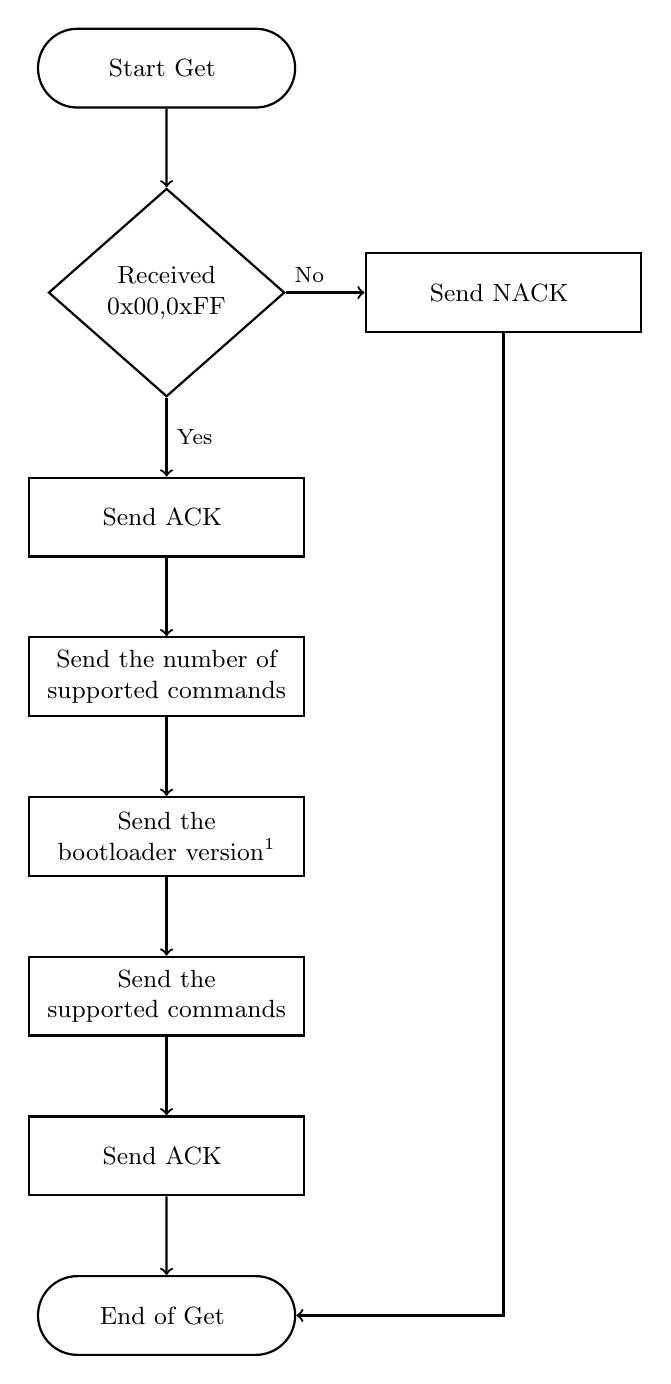
\begin{tikzpicture}[font=\small,thick]
 
\node[draw,
    rounded rectangle,
    minimum width=3.5cm,
    minimum height=1cm,
    align=center
] (block1) { Start Get };

\node[draw,
    diamond,
    below=of block1,
    minimum width=3cm,
    minimum height=2cm,
    align=center
] (block2) { Received\\0x00,0xFF };

\node[draw,
    right=of block2,
    minimum width=3.5cm,
    minimum height=1cm,
    align=center
] (block3N) { Send NACK };

\node[draw,
    below=of block2,
    minimum width=3.5cm,
    minimum height=1cm,
    align=center
] (block3Y) { Send ACK };

\node[draw,
    below=of block3Y,
    minimum width=3.5cm,
    minimum height=1cm,
    align=center
] (block4) { Send the number of\\supported commands };

\node[draw,
    below=of block4,
    minimum width=3.5cm,
    minimum height=1cm,
    align=center
] (block5) { Send the\\bootloader version\footnotemark };

\node[draw,
    below=of block5,
    minimum width=3.5cm,
    minimum height=1cm,
    align=center
] (block6) { Send the\\supported commands };

\node[draw,
    below=of block6,
    minimum width=3.5cm,
    minimum height=1cm,
    align=center
] (block7) { Send ACK };
 
\node[draw,
    rounded rectangle,
    below=of block7,
    minimum width=3.5cm,
    minimum height=1cm,
    align=center
] (block8) { End of Get };

\draw[->] (block1) -- (block2);

\draw[->] (block2) -- (block3Y) node [pos=0.5,right,font=\footnotesize] { Yes };
\draw[->] (block2) -- (block3N) node [pos=0.3,above,font=\footnotesize] { No };

\draw[->] (block3Y) -- (block4);
\draw[->] (block4) -- (block5);
\draw[->] (block5) -- (block6);
\draw[->] (block6) -- (block7);
\draw[->] (block7) -- (block8);

\draw[->] (block3N) |- (block8);

\end{tikzpicture}}}
\footnotetext{The version is represented by a single byte, where MSB nibble represents the major version number, while the LSB nibble represents the minor version number. The version byte can be adjusted by setting the Makefile directive \docVarName{VERSION}}

\clearpage
\subsection{Get Version} \label{cmd:getVersion}

\marginlabel{\captionof{figure}{Get version CMD Flow Diagram}\label{fig:cmd:getVersion}}
\raisebox{-\height}{\scalebox{0.7}{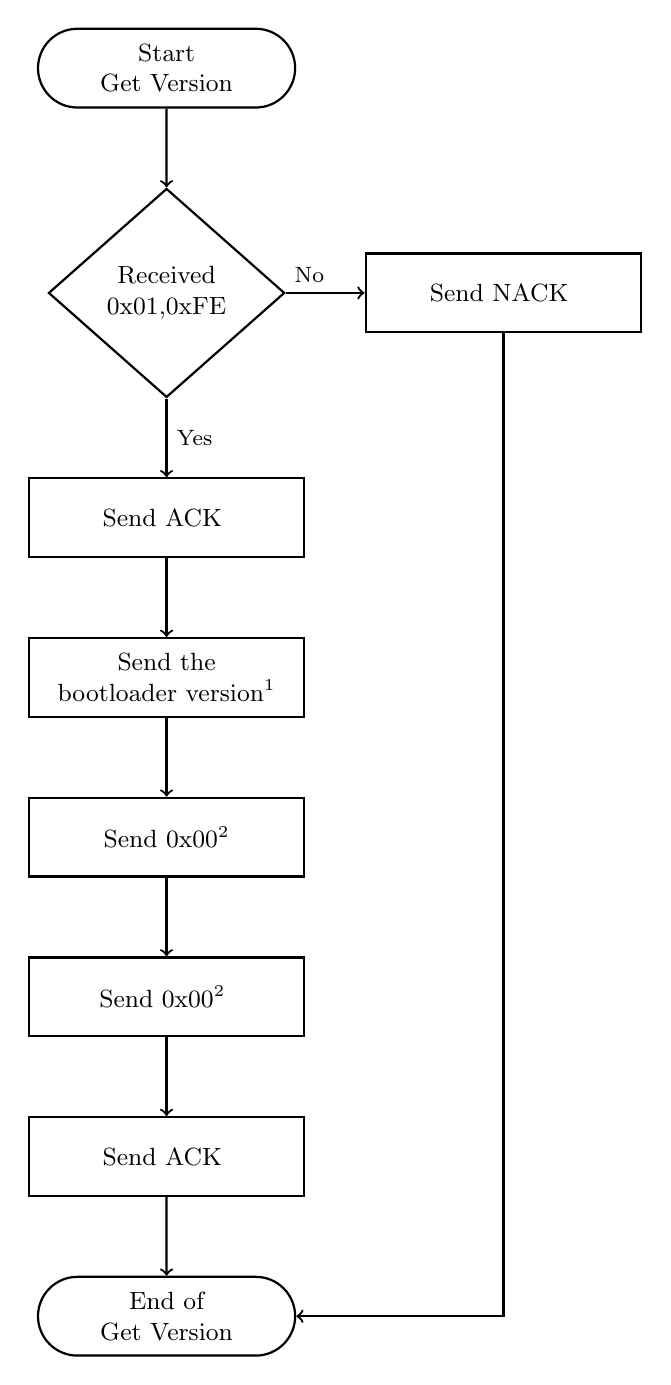
\begin{tikzpicture}[font=\small,thick]
 
\node[draw,
    rounded rectangle,
    minimum width=3.5cm,
    minimum height=1cm,
    align=center
] (block1) { Start\\Get Version };

\node[draw,
    diamond,
    below=of block1,
    minimum width=3cm,
    minimum height=2cm,
    align=center
] (block2) { Received\\0x01,0xFE };

\node[draw,
    right=of block2,
    minimum width=3.5cm,
    minimum height=1cm,
    align=center
] (block3N) { Send NACK };

\node[draw,
    below=of block2,
    minimum width=3.5cm,
    minimum height=1cm,
    align=center
] (block3Y) { Send ACK };

\node[draw,
    below=of block3Y,
    minimum width=3.5cm,
    minimum height=1cm,
    align=center
] (block4) { Send the\\bootloader version\footnotemark };

\node[draw,
    below=of block4,
    minimum width=3.5cm,
    minimum height=1cm,
    align=center
] (block5) { Send 0x00\footnotemark };

\node[draw,
    below=of block5,
    minimum width=3.5cm,
    minimum height=1cm,
    align=center
] (block6) { Send 0x00\footnotemark[\value{footnote}] };

\node[draw,
    below=of block6,
    minimum width=3.5cm,
    minimum height=1cm,
    align=center
] (block7) { Send ACK };
 
\node[draw,
    rounded rectangle,
    below=of block7,
    minimum width=3.5cm,
    minimum height=1cm,
    align=center
] (block8) { End of\\Get Version };

\draw[->] (block1) -- (block2);

\draw[->] (block2) -- (block3Y) node [pos=0.5,right,font=\footnotesize] { Yes };
\draw[->] (block2) -- (block3N) node [pos=0.3,above,font=\footnotesize] { No };

\draw[->] (block3Y) -- (block4);
\draw[->] (block4) -- (block5);
\draw[->] (block5) -- (block6);
\draw[->] (block6) -- (block7);
\draw[->] (block7) -- (block8);

\draw[->] (block3N) |- (block8);

\end{tikzpicture}}}
\addtocounter{footnote}{-1}
\footnotetext{The version is represented by a single byte, where MSB nibble represents the major version number, while the LSB nibble represents the minor version number. The version byte can be adjusted by setting the Makefile directive \docVarName{VERSION}}
\addtocounter{footnote}{+1}
\footnotetext{STM bootloader protocol defines two Option Bytes, here the option bytes are fixed to 0x00}


\clearpage
\subsection{Get ID} \label{cmd:getID}

\marginlabel{\captionof{figure}{Get ID CMD Flow Diagram}\label{fig:cmd:getID}}
\raisebox{-\height}{\scalebox{0.7}{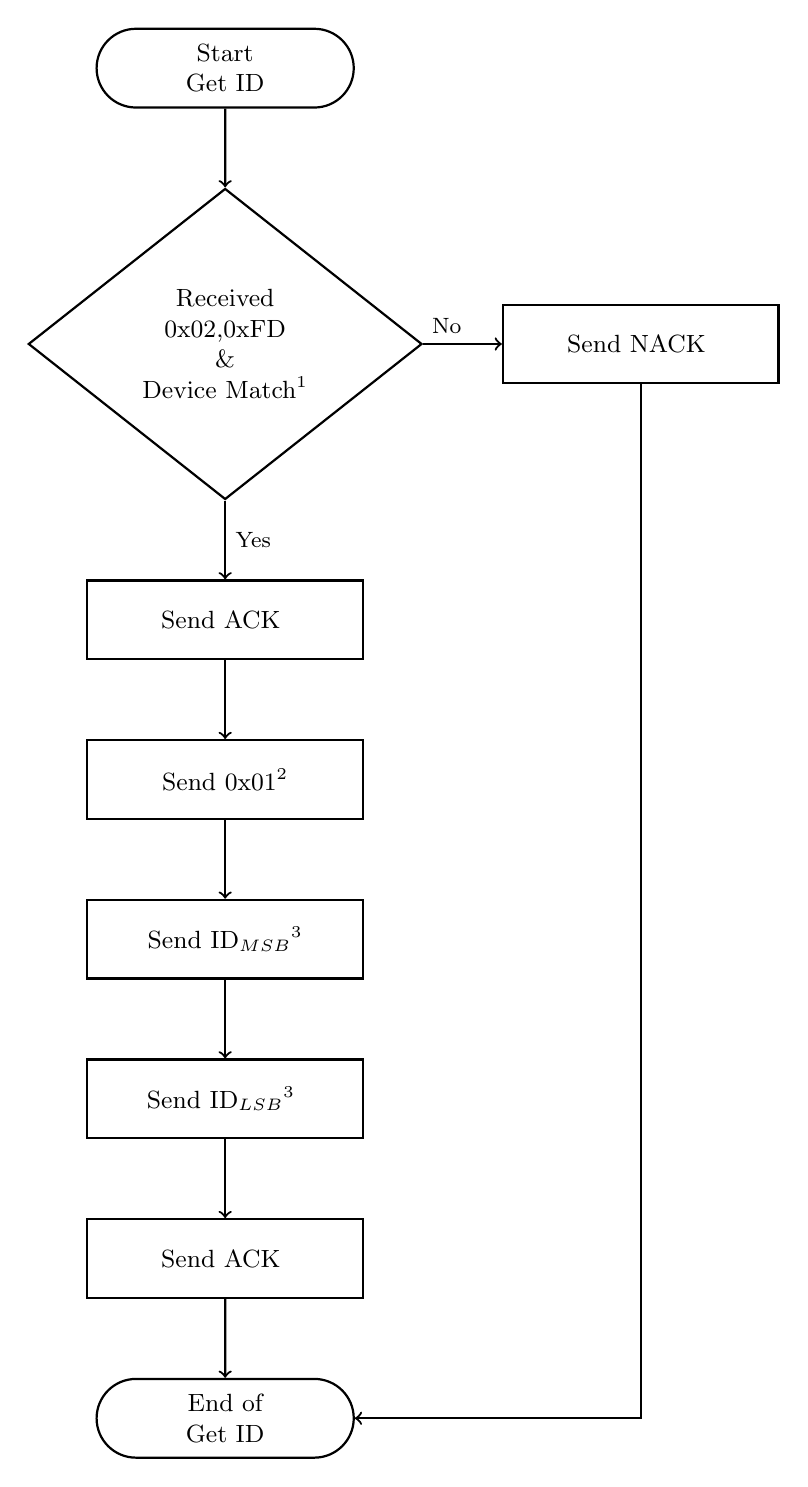
\begin{tikzpicture}[font=\small,thick]
 
\node[draw,
    rounded rectangle,
    minimum width=3.5cm,
    minimum height=1cm,
    align=center
] (block1) { Start\\Get ID };

\node[draw,
    diamond,
    below=of block1,
    minimum width=5cm,
    minimum height=3cm,
    align=center
] (block2) { Received\\0x02,0xFD\\\&\\Device Match\footnotemark };

\node[draw,
    right=of block2,
    minimum width=3.5cm,
    minimum height=1cm,
    align=center
] (block3N) { Send NACK };

\node[draw,
    below=of block2,
    minimum width=3.5cm,
    minimum height=1cm,
    align=center
] (block3Y) { Send ACK };

\node[draw,
    below=of block3Y,
    minimum width=3.5cm,
    minimum height=1cm,
    align=center
] (block4) { Send 0x01\footnotemark };

\node[draw,
    below=of block4,
    minimum width=3.5cm,
    minimum height=1cm,
    align=center
] (block5) { Send ID$_{MSB}$\footnotemark };

\node[draw,
    below=of block5,
    minimum width=3.5cm,
    minimum height=1cm,
    align=center
] (block6) { Send ID$_{LSB}$\footnotemark[\value{footnote}] };

\node[draw,
    below=of block6,
    minimum width=3.5cm,
    minimum height=1cm,
    align=center
] (block7) { Send ACK };
 
\node[draw,
    rounded rectangle,
    below=of block7,
    minimum width=3.5cm,
    minimum height=1cm,
    align=center
] (block8) { End of\\Get ID };

\draw[->] (block1) -- (block2);

\draw[->] (block2) -- (block3Y) node [pos=0.5,right,font=\footnotesize] { Yes };
\draw[->] (block2) -- (block3N) node [pos=0.3,above,font=\footnotesize] { No };

\draw[->] (block3Y) -- (block4);
\draw[->] (block4) -- (block5);
\draw[->] (block5) -- (block6);
\draw[->] (block6) -- (block7);
\draw[->] (block7) -- (block8);

\draw[->] (block3N) |- (block8);

\end{tikzpicture}}}
\addtocounter{footnote}{-2}
\footnotetext{The additional check is added to check if bootloader configuration match the device where it is executed}
\addtocounter{footnote}{+1}
\footnotetext{The first byte is fixed to 0x01 for STM32 devices}
\addtocounter{footnote}{+1}
\footnotetext{ID is sent MSB-first, the emulated device bootloader can be selected by the Makefile variable \docVarName{DEVICE} -- see Section \ref{sec:supportedDevices}}

\clearpage
\subsection{Read Memory} \label{cmd:readMem}

\marginlabel{\captionof{figure}{Read Memory CMD Flow Diagram}\label{fig:cmd:readMem}}
\raisebox{-\height}{\scalebox{0.6}{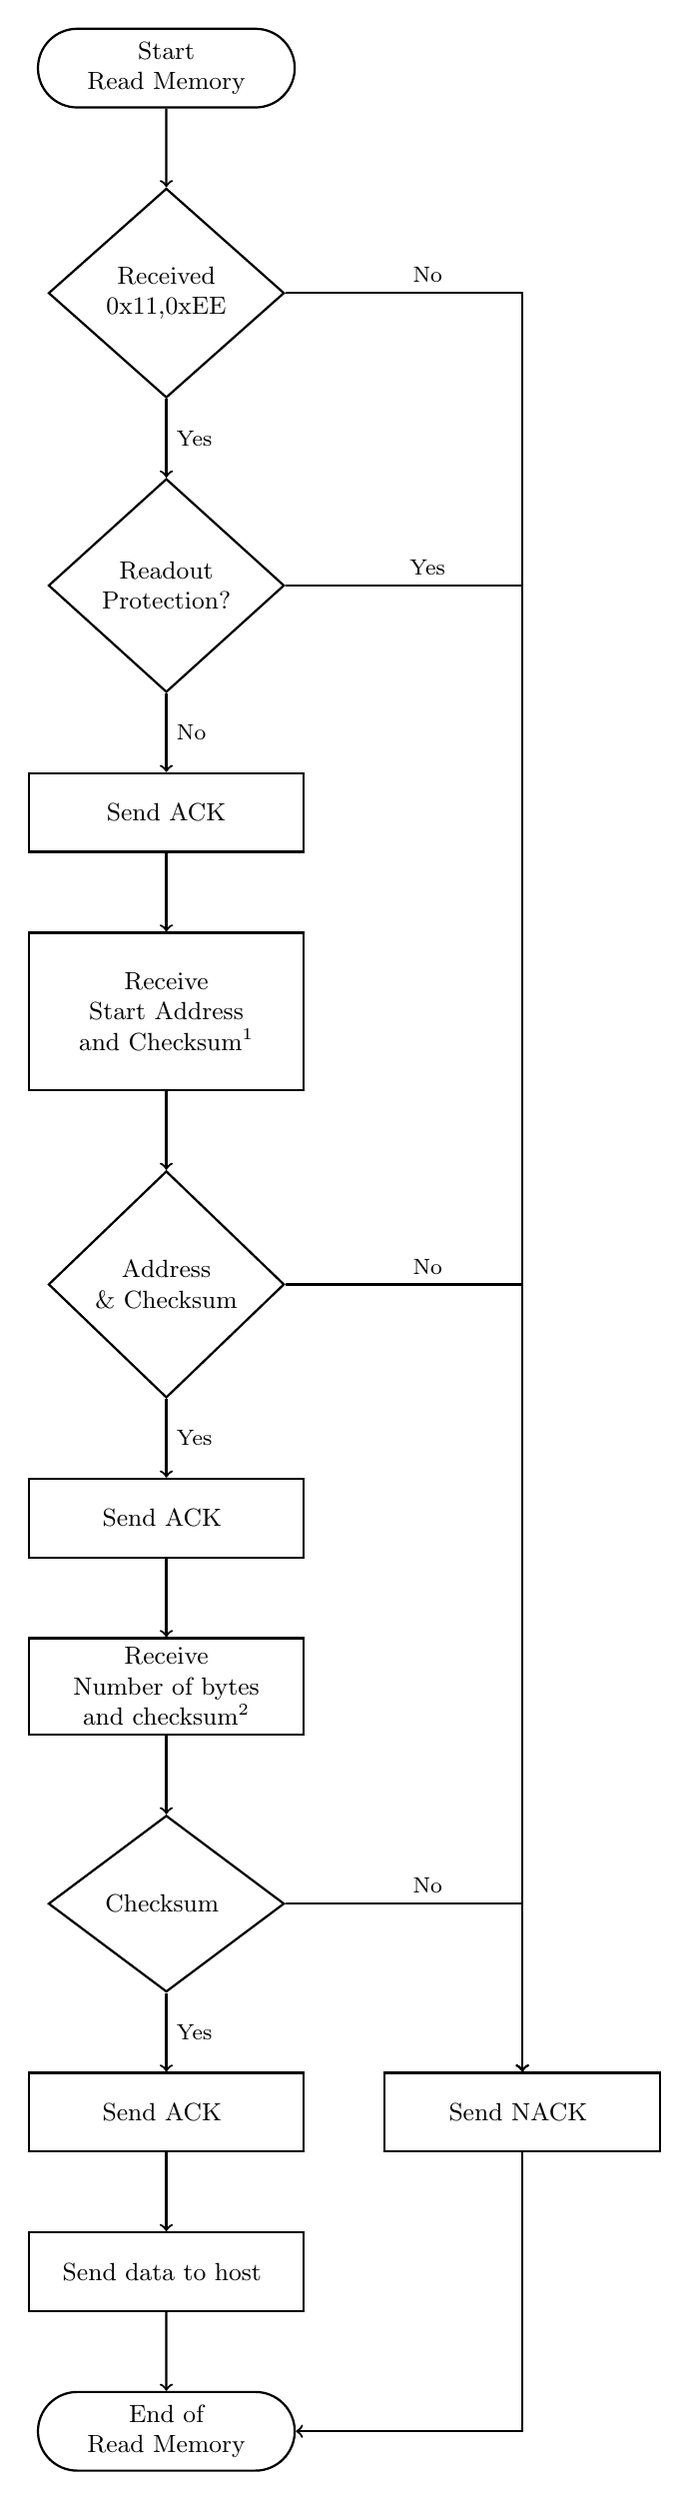
\begin{tikzpicture}[font=\small,thick]
 
\node[draw,
    rounded rectangle,
    minimum width=3.5cm,
    minimum height=1cm,
    align=center
] (block1) { Start\\Read Memory };

\node[draw,
    diamond,
    below=of block1,
    minimum width=3cm,
    minimum height=2cm,
    align=center
] (block2) { Received\\0x11,0xEE };

\node[draw,
    diamond,
    below=of block2,
    minimum width=3cm,
    minimum height=2cm,
    align=center
] (block3Y) { Readout\\Protection? };

\node[draw,
    below=of block3Y,
    minimum width=3.5cm,
    minimum height=1cm,
    align=center
] (block3YN) { Send ACK};

\node[draw,
    below=of block3YN,
    minimum width=3.5cm,
    minimum height=2cm,
    align=center
] (block4) { Receive\\Start Address\\and Checksum\footnotemark };

\node[draw,
    diamond,
    below=of block4,
    minimum width=3cm,
    minimum height=2cm,
    align=center
] (block5) { Address\\\& Checksum };

\node[draw,
    below=of block5,
    minimum width=3.5cm,
    minimum height=1cm,
    align=center
] (block6) { Send ACK };

\node[draw,
    below=of block6,
    minimum width=3.5cm,
    minimum height=1cm,
    align=center
] (block7) { Receive\\Number of bytes\\and checksum\footnotemark };
 
\node[draw,
    diamond,
    below=of block7,
    minimum width=3cm,
    minimum height=2cm,
    align=center
] (block8) { Checksum };
 
\node[draw,
    below=of block8,
    minimum width=3.5cm,
    minimum height=1cm,
    align=center
] (block9) { Send ACK };

\node[draw,
    right=of block9,
    minimum width=3.5cm,
    minimum height=1cm,
    align=center
] (block9N) { Send NACK };

\node[draw,
    below=of block9,
    minimum width=3.5cm,
    minimum height=1cm,
    align=center
] (block10) { Send data to host };
 
\node[draw,
    rounded rectangle,
    below=of block10,
    minimum width=3.5cm,
    minimum height=1cm,
    align=center
] (block11) { End of\\Read Memory };

\draw[->] (block1) -- (block2);

\draw[->] (block2) -- (block3Y) node [pos=0.5,right,font=\footnotesize] { Yes };
\draw[->] (block2) -| (block9N) node [pos=0.3,above,font=\footnotesize] { No };

\draw[->] (block3Y) -- (block3YN) node [pos=0.5,right,font=\footnotesize] { No };
\draw[->] (block3Y) -| (block9N) node [pos=0.3,above,font=\footnotesize] { Yes };

\draw[->] (block3YN) -- (block4);
\draw[->] (block4) -- (block5);
\draw[->] (block5) -- (block6) node [pos=0.5,right,font=\footnotesize] { Yes };
\draw[->] (block5) -| (block9N) node [pos=0.3,above,font=\footnotesize] { No };

\draw[->] (block6) -- (block7);
\draw[->] (block7) -- (block8);
\draw[->] (block8) -- (block9) node [pos=0.5,right,font=\footnotesize] { Yes };
\draw[->] (block8) -| (block9N) node [pos=0.3,above,font=\footnotesize] { No };

\draw[->] (block9) -- (block10);
\draw[->] (block10) -- (block11);

\draw[->] (block9N) |- (block11);

\end{tikzpicture}}}
\addtocounter{footnote}{-1}
\footnotetext{4-byte address is received MSB-first, and the checksum is XOR of address bytes}
\addtocounter{footnote}{+1}
\footnotetext{Number of bytes - 1; the max value of this byte is 255 meaning 256 bytes will be sent; checksum is the complement to the number of bytes}

\clearpage
\subsection{Go} \label{cmd:go}

\marginlabel{\captionof{figure}{Go CMD Flow Diagram}\label{fig:cmd:go}}
\raisebox{-\height}{\scalebox{0.7}{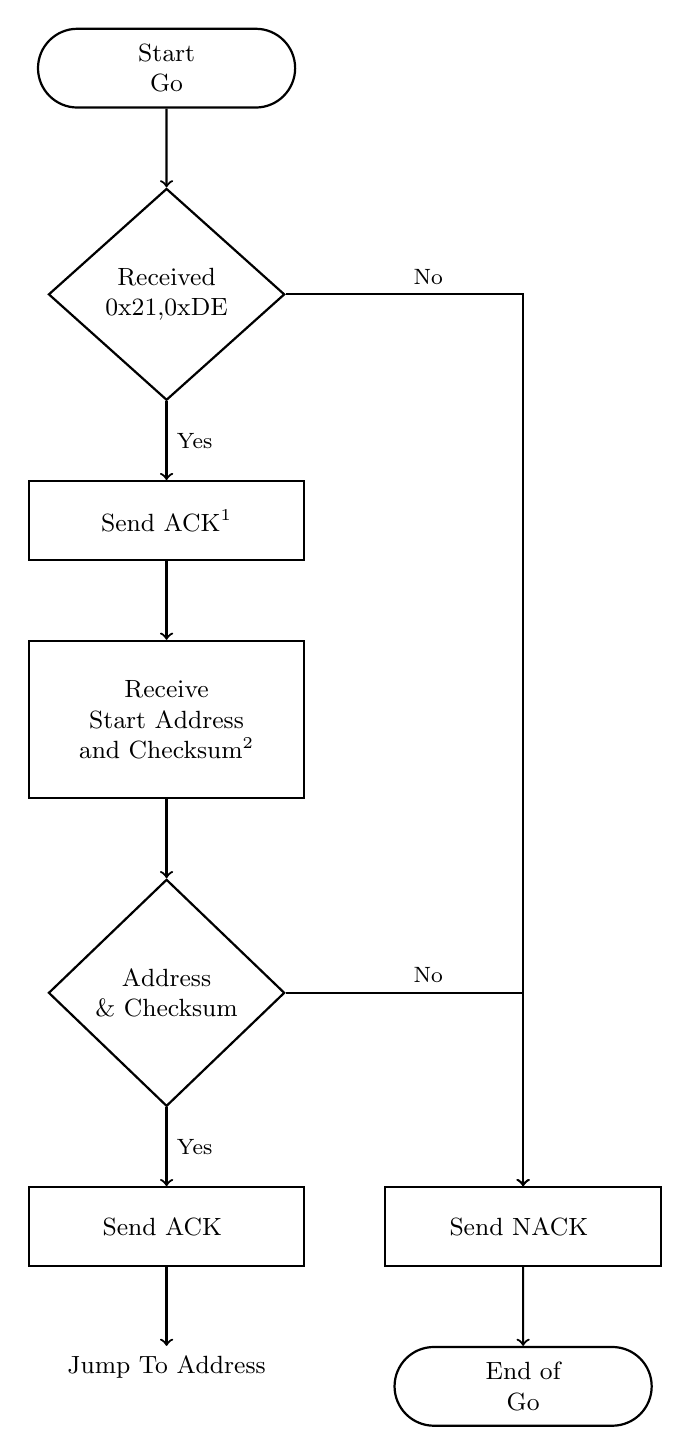
\begin{tikzpicture}[font=\small,thick]
 
\node[draw,
    rounded rectangle,
    minimum width=3.5cm,
    minimum height=1cm,
    align=center
] (block1) { Start\\Go };

\node[draw,
    diamond,
    below=of block1,
    minimum width=3cm,
    minimum height=2cm,
    align=center
] (block2) { Received\\0x21,0xDE };

\node[draw,
    below=of block2,
    minimum width=3.5cm,
    minimum height=1cm,
    align=center
] (block3Y) { Send ACK\footnotemark };

\node[draw,
    below=of block3Y,
    minimum width=3.5cm,
    minimum height=2cm,
    align=center
] (block4) { Receive\\Start Address\\and Checksum\footnotemark };

\node[draw,
    diamond,
    below=of block4,
    minimum width=3cm,
    minimum height=2cm,
    align=center
] (block5) { Address\\\& Checksum };

\node[draw,
    below=of block5,
    minimum width=3.5cm,
    minimum height=1cm,
    align=center
] (block6) { Send ACK };

\node[draw,
    right=of block6,
    minimum width=3.5cm,
    minimum height=1cm,
    align=center
] (block6N) { Send NACK };

 
\node[draw,
    rounded rectangle,
    below=of block6N,
    minimum width=3.5cm,
    minimum height=1cm,
    align=center
] (block7) { End of\\Go };

\node[below=of block6, fill=white] (blockJumpAddr) {Jump To Address};

\draw[->] (block1) -- (block2);

\draw[->] (block2) -- (block3Y) node [pos=0.5,right,font=\footnotesize] { Yes };
\draw[->] (block2) -| (block6N) node [pos=0.3,above,font=\footnotesize] { No };

\draw[->] (block3Y) -- (block4);
\draw[->] (block4) -- (block5);
\draw[->] (block5) -- (block6) node [pos=0.5,right,font=\footnotesize] { Yes };
\draw[->] (block5) -| (block6N) node [pos=0.3,above,font=\footnotesize] { No };
\draw[->] (block6) -- (blockJumpAddr);

\draw[->] (block6N) -- (block7);

\end{tikzpicture}}}
\addtocounter{footnote}{-1}
\footnotetext{Read protection is not checked, ACK is always sent}
\addtocounter{footnote}{+1}
\footnotetext{4-byte address is received MSB-first, and the checksum is XOR of address bytes}
\addtocounter{footnote}{+1}

\clearpage
\subsection{Write Memory} \label{cmd:writeMem}

\marginlabel{\captionof{figure}{Write Memory CMD Flow Diagram}\label{fig:cmd:writeMem}}
\raisebox{-\height}{\scalebox{0.6}{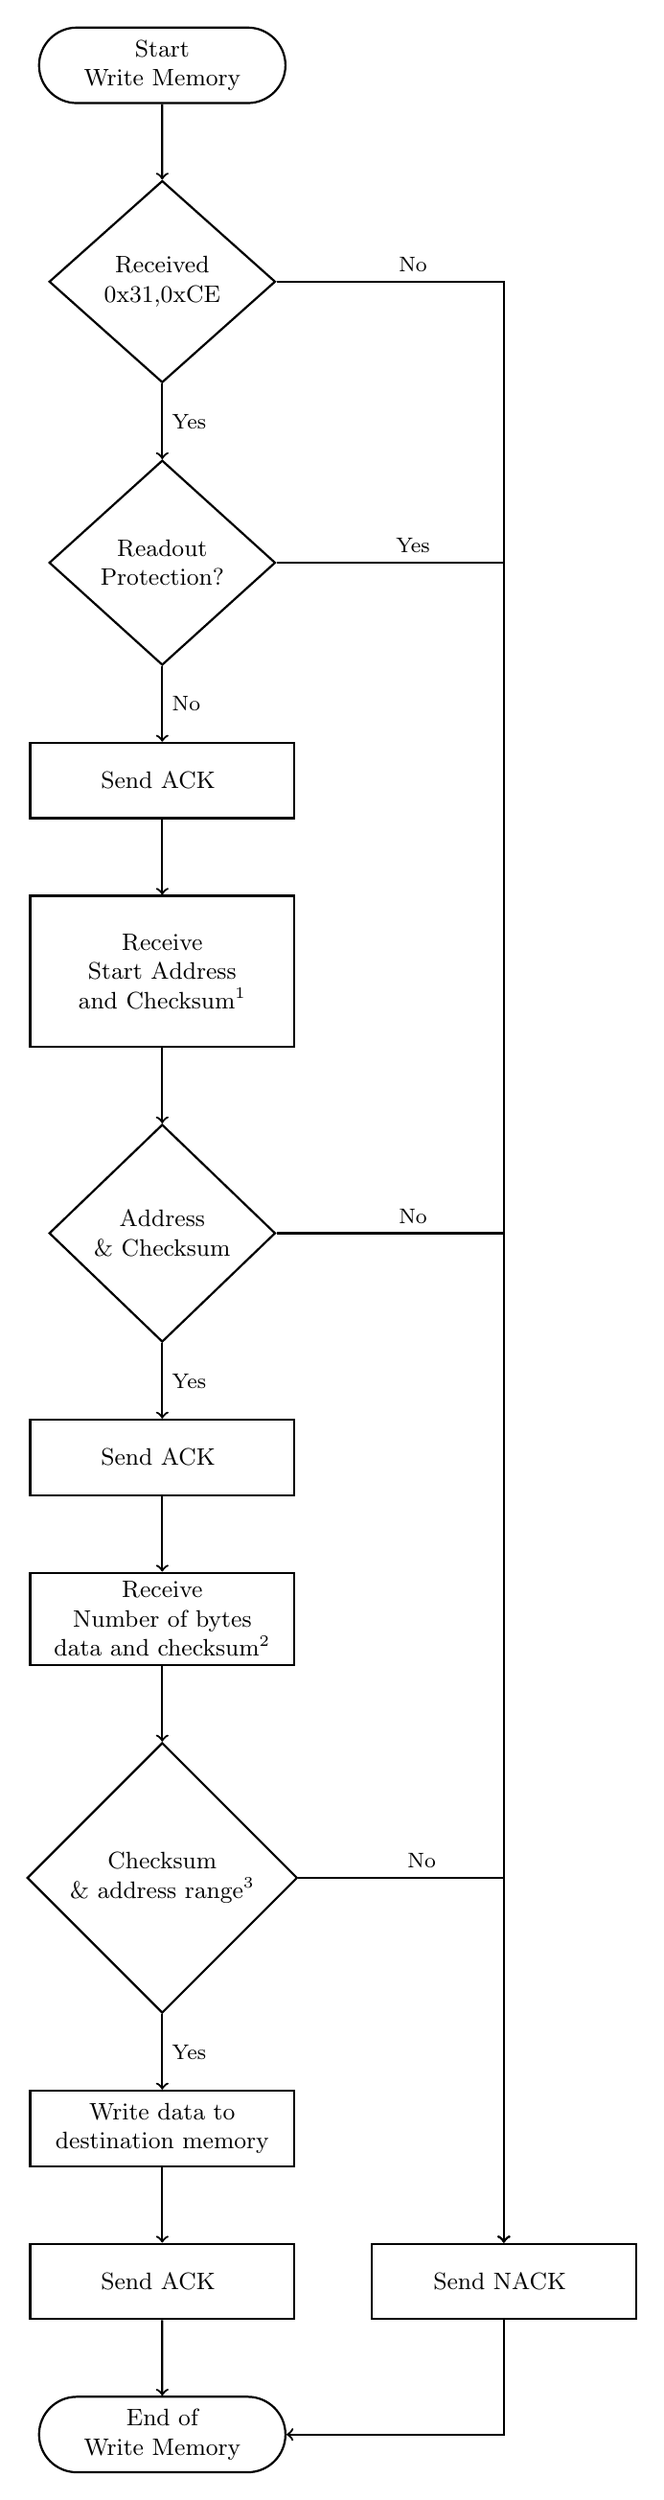
\begin{tikzpicture}[font=\small,thick]
 
\node[draw,
    rounded rectangle,
    minimum width=3.5cm,
    minimum height=1cm,
    align=center
] (block1) { Start\\Write Memory };

\node[draw,
    diamond,
    below=of block1,
    minimum width=3cm,
    minimum height=2cm,
    align=center
] (block2) { Received\\0x31,0xCE };

\node[draw,
    diamond,
    below=of block2,
    minimum width=3cm,
    minimum height=2cm,
    align=center
] (block3Y) { Readout\\Protection? };

\node[draw,
    below=of block3Y,
    minimum width=3.5cm,
    minimum height=1cm,
    align=center
] (block3YN) { Send ACK };

\node[draw,
    below=of block3YN,
    minimum width=3.5cm,
    minimum height=2cm,
    align=center
] (block4) { Receive\\Start Address\\and Checksum\footnotemark };

\node[draw,
    diamond,
    below=of block4,
    minimum width=3cm,
    minimum height=2cm,
    align=center
] (block5) { Address\\\& Checksum };

\node[draw,
    below=of block5,
    minimum width=3.5cm,
    minimum height=1cm,
    align=center
] (block6) { Send ACK };

\node[draw,
    below=of block6,
    minimum width=3.5cm,
    minimum height=1cm,
    align=center
] (block7) { Receive\\Number of bytes\\data and checksum\footnotemark };
 
\node[draw,
    diamond,
    below=of block7,
    minimum width=3cm,
    minimum height=2cm,
    align=center
] (block8) { Checksum\\\& address range\footnotemark };

 
\node[draw,
    below=of block8,
    minimum width=3.5cm,
    minimum height=1cm,
    align=center
] (block9) { Write data to\\destination memory };
 
\node[draw,
    below=of block9,
    minimum width=3.5cm,
    minimum height=1cm,
    align=center
] (block10) { Send ACK };

\node[draw,
    right=of block10,
    minimum width=3.5cm,
    minimum height=1cm,
    align=center
] (block9N) { Send NACK };
 
\node[draw,
    rounded rectangle,
    below=of block10,
    minimum width=3.5cm,
    minimum height=1cm,
    align=center
] (block11) { End of\\Write Memory };

\draw[->] (block1) -- (block2);

\draw[->] (block2) -- (block3Y) node [pos=0.5,right,font=\footnotesize] { Yes };
\draw[->] (block2) -| (block9N) node [pos=0.3,above,font=\footnotesize] { No };

\draw[->] (block3Y) -- (block3YN) node [pos=0.5,right,font=\footnotesize] { No };
\draw[->] (block3Y) -| (block9N) node [pos=0.3,above,font=\footnotesize] { Yes };

\draw[->] (block3YN) -- (block4);
\draw[->] (block4) -- (block5);
\draw[->] (block5) -- (block6) node [pos=0.5,right,font=\footnotesize] { Yes };
\draw[->] (block5) -| (block9N) node [pos=0.3,above,font=\footnotesize] { No };

\draw[->] (block6) -- (block7);
\draw[->] (block7) -- (block8);
\draw[->] (block8) -- (block9) node [pos=0.5,right,font=\footnotesize] { Yes };
\draw[->] (block8) -| (block9N) node [pos=0.3,above,font=\footnotesize] { No };

\draw[->] (block9) -- (block10);
\draw[->] (block10) -- (block11);

\draw[->] (block9N) |- (block11);

\end{tikzpicture}}}
\addtocounter{footnote}{-2}
\footnotetext{4-byte address is received MSB-first, and the checksum is XOR of address bytes}
\addtocounter{footnote}{+1}
\footnotetext{Number of bytes - 1; the max value of this byte is 255 meaning 256 bytes will be received, while the value must be multiple of four; checksum is computed as a XOR of the length and all received data bytes}
\addtocounter{footnote}{+1}
\footnotetext{Option byte writes are currently not supported}
  


\clearpage
\subsection{Erase Memory} \label{cmd:eraseMem}

\marginlabel{\captionof{figure}{Erase Memory CMD Flow Diagram}\label{fig:cmd:eraseMem}}
\raisebox{-\height}{\scalebox{0.7}{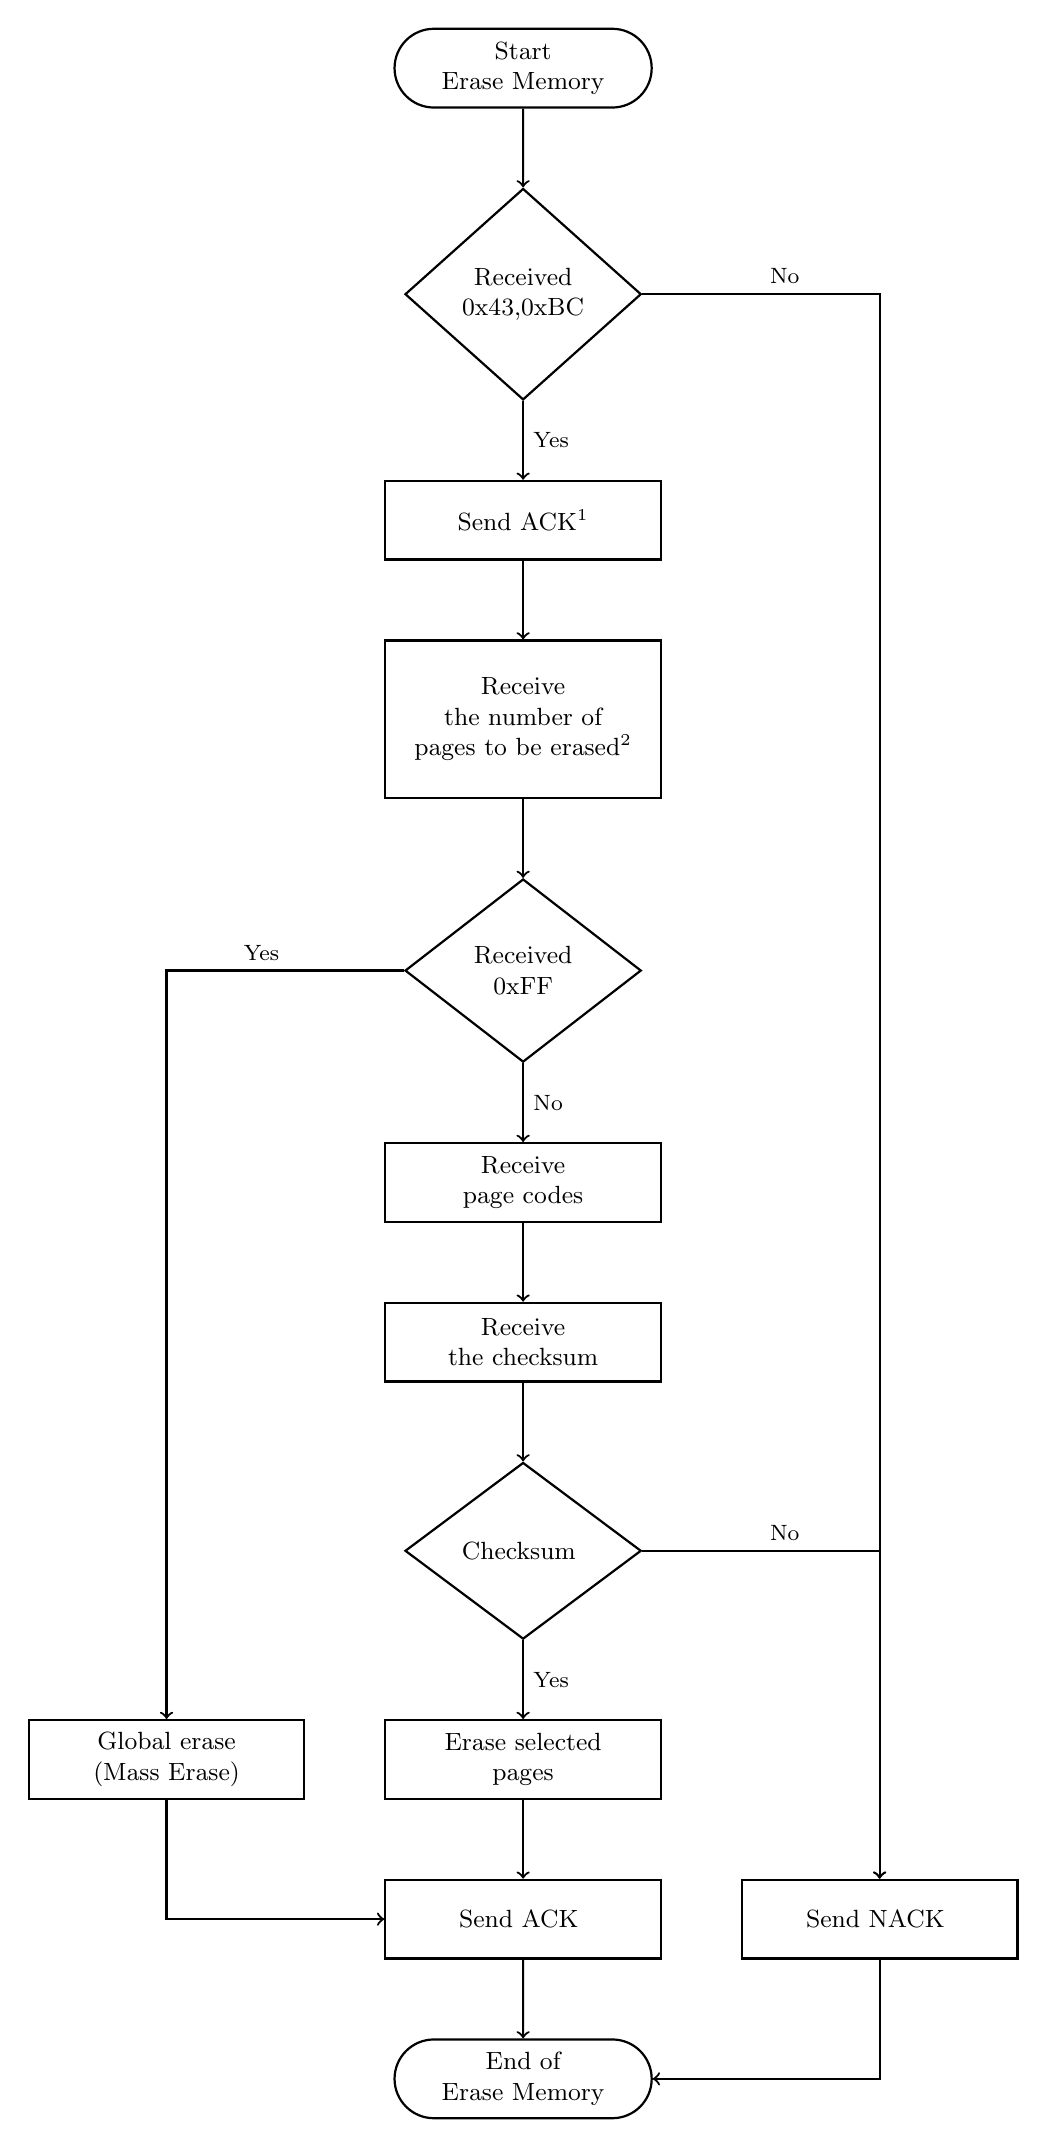
\begin{tikzpicture}[font=\small,thick]
 
\node[draw,
    rounded rectangle,
    minimum width=3.5cm,
    minimum height=1cm,
    align=center
] (block1) { Start\\Erase Memory };

\node[draw,
    diamond,
    below=of block1,
    minimum width=3cm,
    minimum height=2cm,
    align=center
] (block2) { Received\\0x43,0xBC };

\node[draw,
    below=of block2,
    minimum width=3.5cm,
    minimum height=1cm,
    align=center
] (block3Y) { Send ACK\footnotemark };

\node[draw,
    below=of block3Y,
    minimum width=3.5cm,
    minimum height=2cm,
    align=center
] (block4) { Receive\\the number of\\pages to be erased\footnotemark };

\node[draw,
    diamond,
    below=of block4,
    minimum width=3cm,
    minimum height=2cm,
    align=center
] (block5) { Received\\0xFF };

\node[draw,
    below=of block5,
    minimum width=3.5cm,
    minimum height=1cm,
    align=center
] (block6) { Receive\\page codes };

\node[draw,
    below=of block6,
    minimum width=3.5cm,
    minimum height=1cm,
    align=center
] (block7) { Receive\\the checksum };
 
\node[draw,
    diamond,
    below=of block7,
    minimum width=3cm,
    minimum height=2cm,
    align=center
] (block8) { Checksum };

 
\node[draw,
    below=of block8,
    minimum width=3.5cm,
    minimum height=1cm,
    align=center
] (block9) { Erase selected\\pages };
 
\node[draw,
    left=of block9,
    minimum width=3.5cm,
    minimum height=1cm,
    align=center
] (block6Y) { Global erase\\(Mass Erase) };
 
\node[draw,
    below=of block9,
    minimum width=3.5cm,
    minimum height=1cm,
    align=center
] (block10) { Send ACK };

\node[draw,
    right=of block10,
    minimum width=3.5cm,
    minimum height=1cm,
    align=center
] (block9N) { Send NACK };
 
\node[draw,
    rounded rectangle,
    below=of block10,
    minimum width=3.5cm,
    minimum height=1cm,
    align=center
] (block11) { End of\\Erase Memory };

\draw[->] (block1) -- (block2);

\draw[->] (block2) -- (block3Y) node [pos=0.5,right,font=\footnotesize] { Yes };
\draw[->] (block2) -| (block9N) node [pos=0.3,above,font=\footnotesize] { No };

\draw[->] (block3Y) -- (block4);
\draw[->] (block4) -- (block5);
\draw[->] (block5) -- (block6) node [pos=0.5,right,font=\footnotesize] { No };
\draw[->] (block5) -| (block6Y) node [pos=0.3,above,font=\footnotesize] { Yes };

\draw[->] (block6Y) |- (block10);

\draw[->] (block6) -- (block7);
\draw[->] (block7) -- (block8);
\draw[->] (block8) -- (block9) node [pos=0.5,right,font=\footnotesize] { Yes };
\draw[->] (block8) -| (block9N) node [pos=0.3,above,font=\footnotesize] { No };

\draw[->] (block9) -- (block10);
\draw[->] (block10) -- (block11);

\draw[->] (block9N) |- (block11);

\end{tikzpicture}}}
\addtocounter{footnote}{-1}
\footnotetext{Read protection is not checked, ACK is always sent}
\addtocounter{footnote}{+1}
\footnotetext{Number of pages to be erased decreased by 1; 0xFF is a special value and it starts Mass Erase}


\clearpage
\subsection{Extended Erase Memory} \label{cmd:extEraseMem}

\marginlabel{\captionof{figure}{Extended Erase Memory CMD Flow Diagram}\label{fig:cmd:extEraseMem}}
\raisebox{-\height}{\scalebox{0.7}{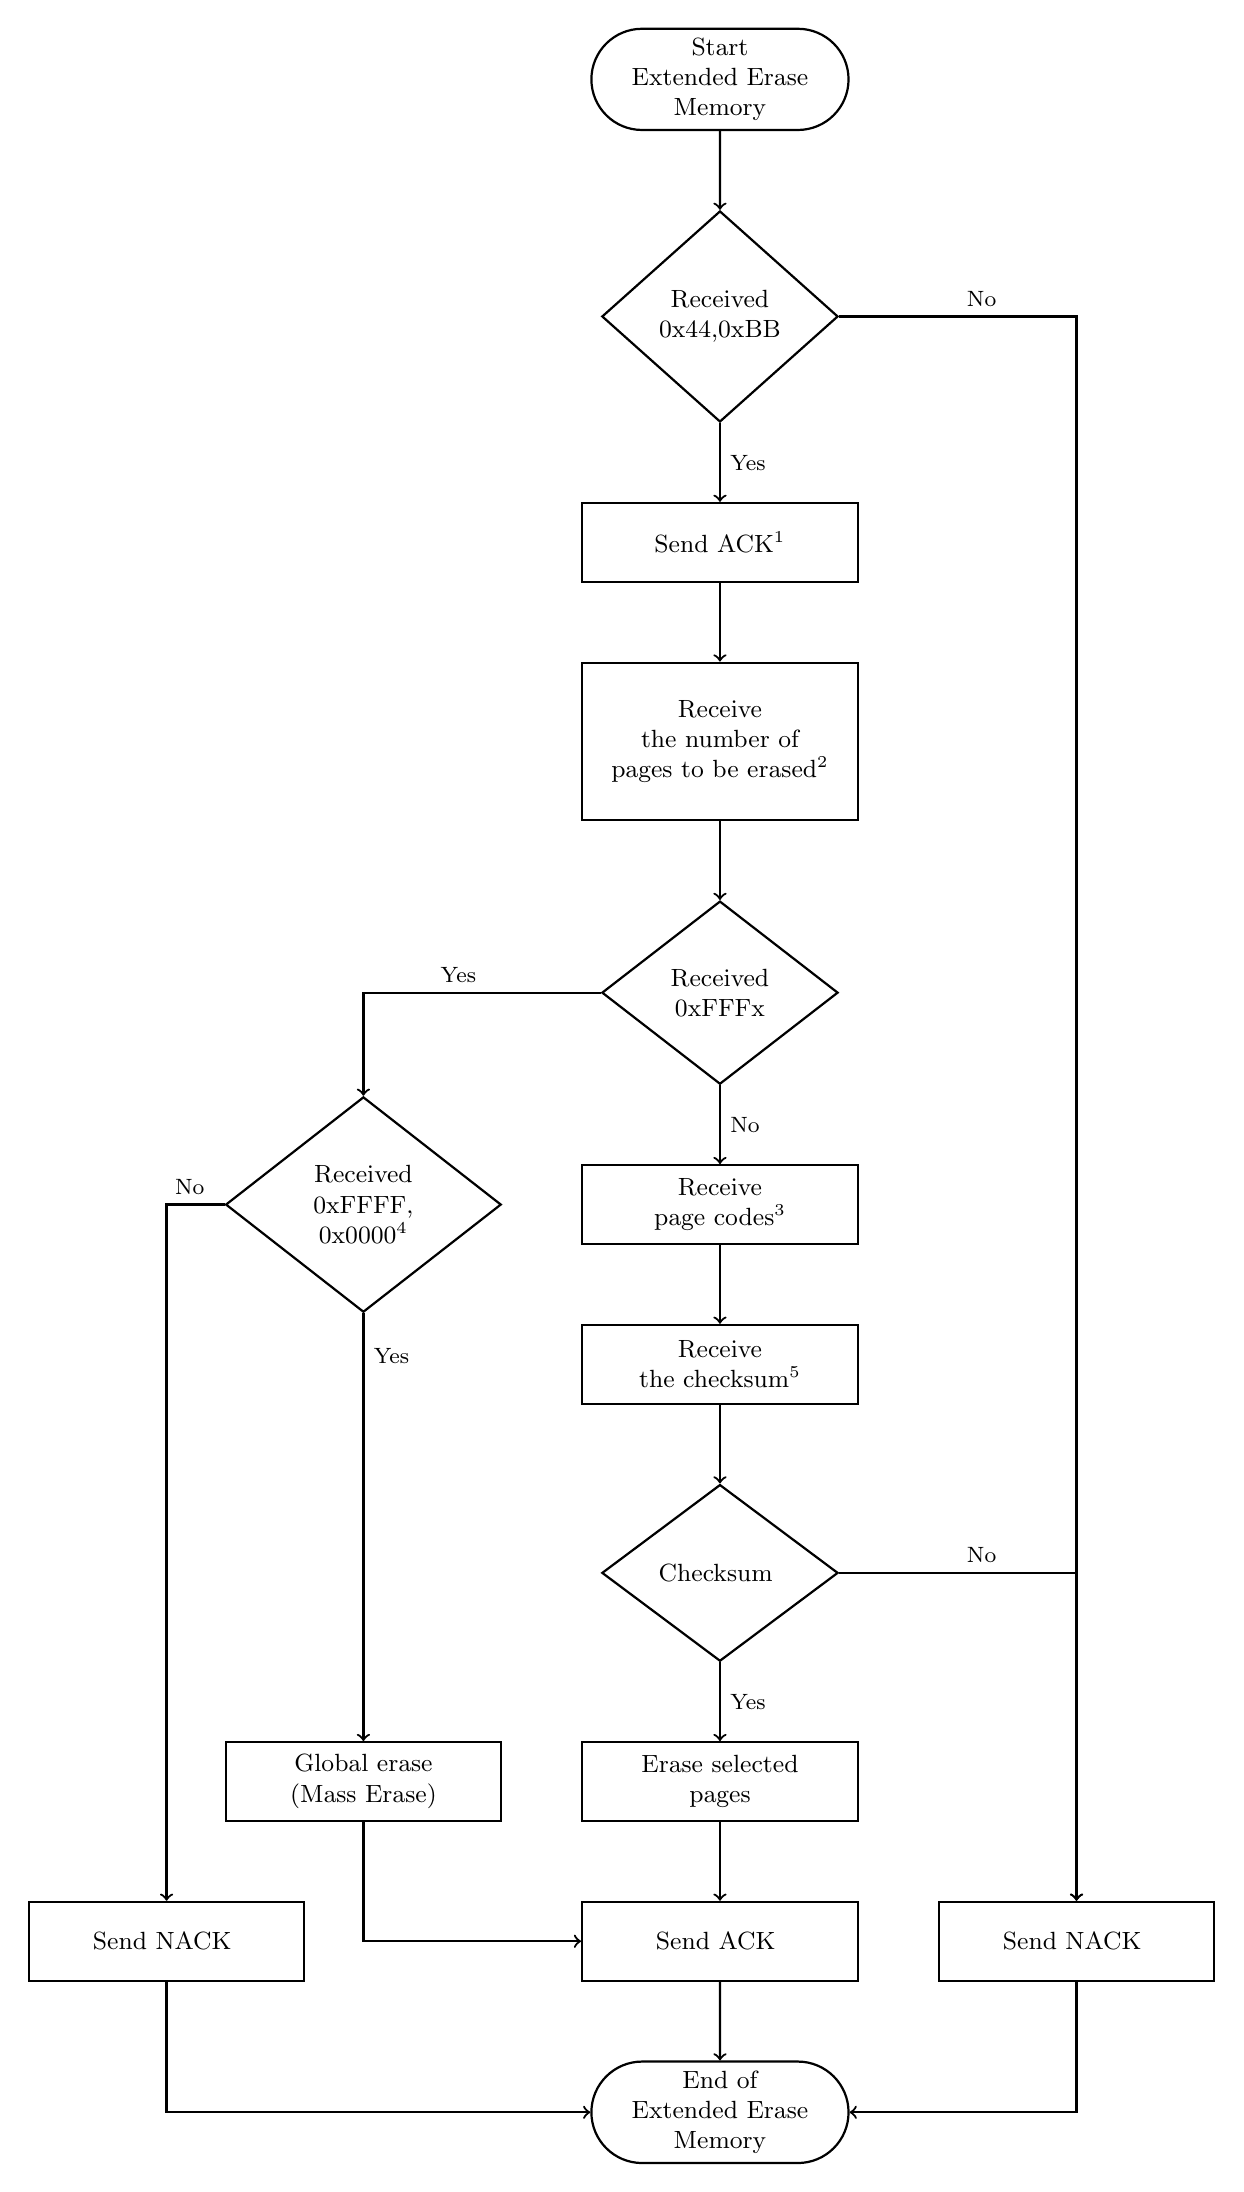
\begin{tikzpicture}[font=\small,thick]
 
\node[draw,
    rounded rectangle,
    minimum width=3.5cm,
    minimum height=1cm,
    align=center
] (block1) { Start\\Extended Erase\\Memory };

\node[draw,
    diamond,
    below=of block1,
    minimum width=3cm,
    minimum height=2cm,
    align=center
] (block2) { Received\\0x44,0xBB };

\node[draw,
    below=of block2,
    minimum width=3.5cm,
    minimum height=1cm,
    align=center
] (block3Y) { Send ACK\footnotemark };

\node[draw,
    below=of block3Y,
    minimum width=3.5cm,
    minimum height=2cm,
    align=center
] (block4) { Receive\\the number of\\pages to be erased\footnotemark };

\node[draw,
    diamond,
    below=of block4,
    minimum width=3cm,
    minimum height=2cm,
    align=center
] (block5) { Received\\0xFFFx };

\node[draw,
    below=of block5,
    minimum width=3.5cm,
    minimum height=1cm,
    align=center
] (block6) { Receive\\page codes\footnotemark };

\node[draw,
    diamond,
    left=of block6,
    minimum width=3.5cm,
    minimum height=2.5cm,
    align=center
] (blockMassYN) { Received\\0xFFFF,\\0x0000\footnotemark };

\node[draw,
    below=of block6,
    minimum width=3.5cm,
    minimum height=1cm,
    align=center
] (block7) { Receive\\the checksum\footnotemark };
 
\node[draw,
    diamond,
    below=of block7,
    minimum width=3cm,
    minimum height=2cm,
    align=center
] (block8) { Checksum };

 
\node[draw,
    below=of block8,
    minimum width=3.5cm,
    minimum height=1cm,
    align=center
] (block9) { Erase selected\\pages };
 
\node[draw,
    left=of block9,
    minimum width=3.5cm,
    minimum height=1cm,
    align=center
] (block6Y) { Global erase\\(Mass Erase) };
 
\node[draw,
    below=of block9,
    minimum width=3.5cm,
    minimum height=1cm,
    align=center
] (block10) { Send ACK };

\node[draw,
    right=of block10,
    minimum width=3.5cm,
    minimum height=1cm,
    align=center
] (block9N) { Send NACK };

\node[draw,
    left=3.5cm of block10,
    minimum width=3.5cm,
    minimum height=1cm,
    align=center
] (blockMassNACK) { Send NACK };
 
\node[draw,
    rounded rectangle,
    below=of block10,
    minimum width=3.5cm,
    minimum height=1cm,
    align=center
] (block11) { End of\\Extended Erase\\Memory };

\draw[->] (block1) -- (block2);

\draw[->] (block2) -- (block3Y) node [pos=0.5,right,font=\footnotesize] { Yes };
\draw[->] (block2) -| (block9N) node [pos=0.3,above,font=\footnotesize] { No };

\draw[->] (block3Y) -- (block4);
\draw[->] (block4) -- (block5);
\draw[->] (block5) -- (block6) node [pos=0.5,right,font=\footnotesize] { No };

\draw[->] (block5) -| (blockMassYN) node [pos=0.3,above,font=\footnotesize] { Yes };
\draw[->] (blockMassYN) -- (block6Y)  node [pos=0.1,right,font=\footnotesize] { Yes };
\draw[->] (blockMassYN) -| (blockMassNACK)  node [pos=0.3,above,font=\footnotesize] { No };

\draw[->] (block6Y) |- (block10);

\draw[->] (block6) -- (block7);
\draw[->] (block7) -- (block8);
\draw[->] (block8) -- (block9) node [pos=0.5,right,font=\footnotesize] { Yes };
\draw[->] (block8) -| (block9N) node [pos=0.3,above,font=\footnotesize] { No };

\draw[->] (block9) -- (block10);
\draw[->] (block10) -- (block11);

\draw[->] (block9N) |- (block11);
\draw[->] (blockMassNACK) |- (block11);

\end{tikzpicture}}}
\addtocounter{footnote}{-4}
\footnotetext{Read protection is not checked, ACK is always sent}
\addtocounter{footnote}{+1}
\footnotetext{Number of pages to be erased encoded on two bytes (MSB-first) decreased by 1 -- maximum is 512 pages; 0xFFFx encode special values (0xFFFF is Mass Erase, while the other values are RFU)}
\addtocounter{footnote}{+1}
\footnotetext{Each page is encoded by two bytes (MSB-first)}
\addtocounter{footnote}{+1}
\footnotetext{Receive 2 bytes (MSB-first) encoding special value and another 2 bytes (MSB-first), as the commandm complement: 0xFFFF code encodes Mass Erase}
\addtocounter{footnote}{+1}
\footnotetext{Checksum is a single byte computed over all bytes received since the number of pages - 1 bytes (included)}

\clearpage
\subsection{Special Command} \label{cmd:special}

\marginlabel{\captionof{figure}{Special CMD Flow Diagram}\label{fig:cmd:special}}
\raisebox{-\height}{\scalebox{0.55}{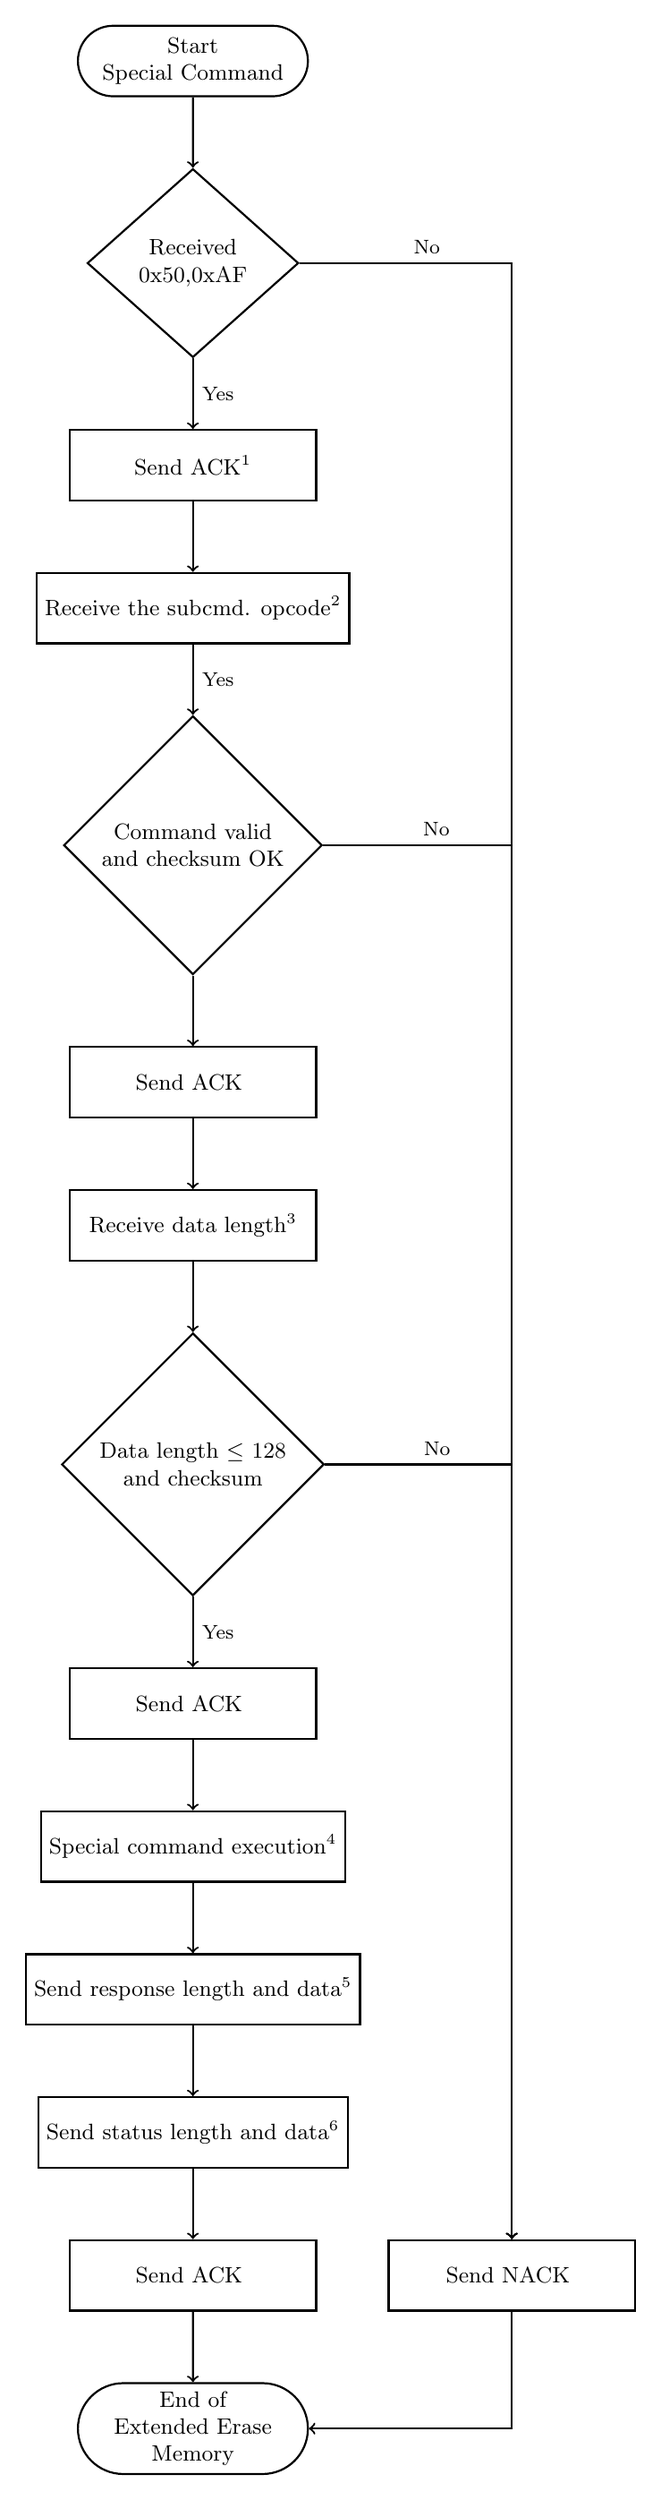
\begin{tikzpicture}[font=\small,thick]
 
\node[draw,
    rounded rectangle,
    minimum width=3.5cm,
    minimum height=1cm,
    align=center
] (block1) { Start\\Special Command };

\node[draw,
    diamond,
    below=of block1,
    minimum width=3cm,
    minimum height=2cm,
    align=center
] (block2) { Received\\0x50,0xAF };

\node[draw,
    below=of block2,
    minimum width=3.5cm,
    minimum height=1cm,
    align=center
] (block3) { Send ACK\footnotemark };

\node[draw,
    below=of block3,
    minimum width=3.5cm,
    minimum height=1cm,
    align=center
] (block4) { Receive the subcmd. opcode\footnotemark };

\node[draw,
    diamond,
    below=of block4,
    minimum width=3cm,
    minimum height=2cm,
    align=center
] (block5) { Command valid\\and checksum OK };

\node[draw,
    below=of block5,
    minimum width=3.5cm,
    minimum height=1cm,
    align=center
] (block6) { Send ACK };

\node[draw,
    below=of block6,
    minimum width=3.5cm,
    minimum height=1cm,
    align=center
] (block7) { Receive data length\footnotemark };
 
\node[draw,
    diamond,
    below=of block7,
    minimum width=3cm,
    minimum height=2cm,
    align=center
] (block8) { Data length $\leq$ 128\\and checksum };
 
\node[draw,
    below=of block8,
    minimum width=3.5cm,
    minimum height=1cm,
    align=center
] (block9) { Send ACK };
 
\node[draw,
    below=of block9,
    minimum width=3.5cm,
    minimum height=1cm,
    align=center
] (block10) { Special command execution\footnotemark };

\node[draw,
    below=of block10,
    minimum width=3.5cm,
    minimum height=1cm,
    align=center
] (block11) { Send response length and data\footnotemark };

\node[draw,
    below=of block11,
    minimum width=3.5cm,
    minimum height=1cm,
    align=center
] (block13) { Send status length and data\footnotemark };
 
 
\node[draw,
    below=of block13,
    minimum width=3.5cm,
    minimum height=1cm,
    align=center
] (block15) { Send ACK };

\node[draw,
    right=of block15,
    minimum width=3.5cm,
    minimum height=1cm,
    align=center
] (block15N) { Send NACK };

\node[draw,
    rounded rectangle,
    below=of block15,
    minimum width=3.5cm,
    minimum height=1cm,
    align=center
] (block16) { End of\\Extended Erase\\Memory };

\draw[->] (block1) -- (block2);

\draw[->] (block2) -- (block3) node [pos=0.5,right,font=\footnotesize] { Yes };
\draw[->] (block2) -| (block15N) node [pos=0.3,above,font=\footnotesize] { No };

\draw[->] (block3) -- (block4);
\draw[->] (block4) -- (block5)node [pos=0.5,right,font=\footnotesize] { Yes };
\draw[->] (block5) -| (block15N) node [pos=0.3,above,font=\footnotesize] { No };

\draw[->] (block5) -- (block6);
\draw[->] (block6) -- (block7);
\draw[->] (block7) -- (block8);
\draw[->] (block8) -- (block9) node [pos=0.5,right,font=\footnotesize] { Yes };
\draw[->] (block8) -| (block15N) node [pos=0.3,above,font=\footnotesize] { No };

\draw[->] (block9) -- (block10);
\draw[->] (block10) -- (block11);
\draw[->] (block11) -- (block13);
\draw[->] (block13) -- (block15);
\draw[->] (block15) -- (block16);
\draw[->] (block15N) |- (block16);


\end{tikzpicture}}}

\addtocounter{footnote}{-5}
\footnotetext{2 bytes, MSB-first + checksum byte}
\addtocounter{footnote}{+1}
\footnotetext{2 bytes, MSB-first + checksum byte}
\addtocounter{footnote}{+1}
\footnotetext{2 bytes, MSB first + checksum byte}
\addtocounter{footnote}{+1}
\footnotetext{Timing depends on the special command nature}
\addtocounter{footnote}{+1}
\footnotetext{2 bytes of response data length, MSB first, no checksum; if length is 0, no data transmitted}
\addtocounter{footnote}{+1}
\footnotetext{2 bytes of status data length, MSB first, no checksum; if length is 0, no data transmitted}


\clearpage
\subsection{Readout Protect} \label{cmd:readProtect}

\marginlabel{\captionof{figure}{Readout Protect CMD Flow Diagram}\label{fig:cmd:readProtect}}
\raisebox{-\height}{\scalebox{0.7}{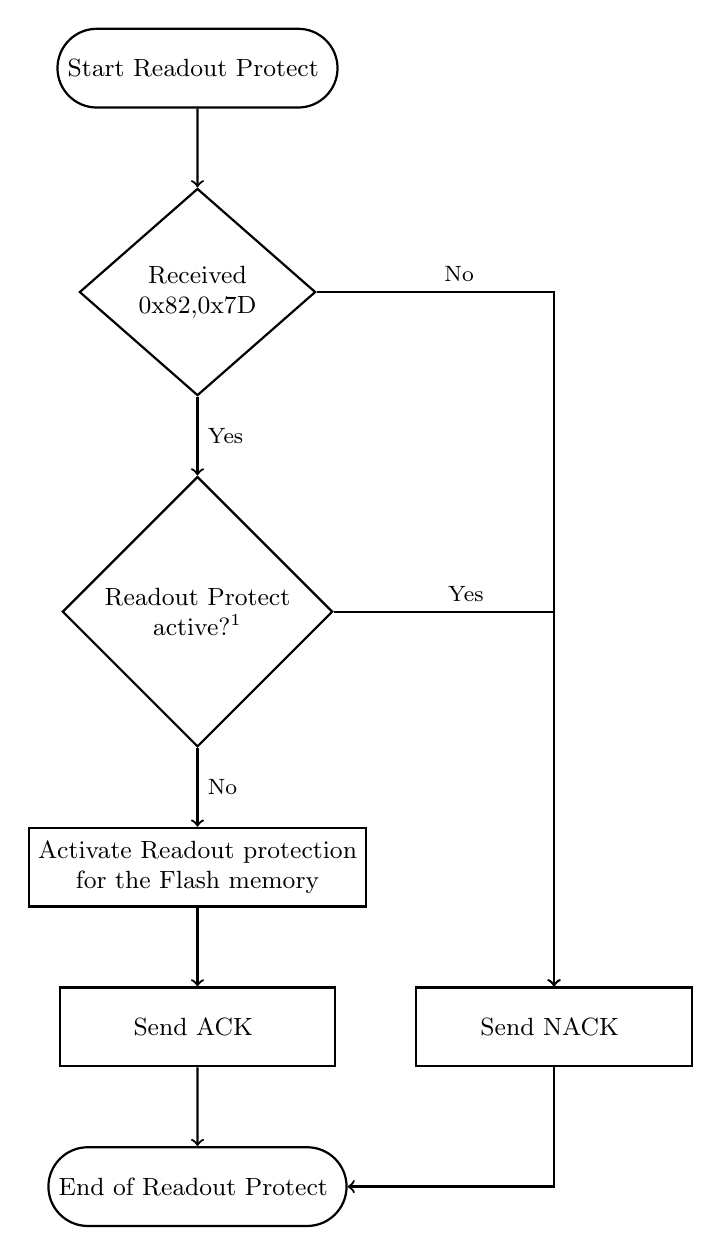
\begin{tikzpicture}[font=\small,thick]
 
\node[draw,
    rounded rectangle,
    minimum width=3.5cm,
    minimum height=1cm,
    align=center
] (block1) { Start Readout Protect };

\node[draw,
    diamond,
    below=of block1,
    minimum width=3cm,
    minimum height=2cm,
    align=center
] (block2) { Received\\0x82,0x7D };

\node[draw,
    diamond,
    below=of block2,
    minimum width=3cm,
    minimum height=2cm,
    align=center
] (block3Y) { Readout Protect\\ active?\footnotemark };

\node[draw,
    below=of block3Y,
    minimum width=3.5cm,
    minimum height=1cm,
    align=center
] (block4) { Activate Readout protection\\for the Flash memory };

\node[draw,
    below=of block4,
    minimum width=3.5cm,
    minimum height=1cm,
    align=center
] (block5) { Send ACK };

\node[draw,
    right=of block5,
    minimum width=3.5cm,
    minimum height=1cm,
    align=center
] (block3N) { Send NACK };
 
\node[draw,
    rounded rectangle,
    below=of block5,
    minimum width=3.5cm,
    minimum height=1cm,
    align=center
] (block6) { End of Readout Protect };

\draw[->] (block1) -- (block2);

\draw[->] (block2) -- (block3Y) node [pos=0.5,right,font=\footnotesize] { Yes };
\draw[->] (block2) -| (block3N) node [pos=0.3,above,font=\footnotesize] { No };

\draw[->] (block3Y) -- (block4) node [pos=0.5,right,font=\footnotesize] { No };
\draw[->] (block3Y) -| (block3N) node [pos=0.3,above,font=\footnotesize] { Yes };

\draw[->] (block4) -- (block5);

\draw[->] (block5) -- (block6);
\draw[->] (block3N) |- (block6);

\end{tikzpicture}}}
\footnotetext{If readout protection is active, NACK is returned -- this allows to test if readout protection was active or not.}

\clearpage
\subsection{Readout Unprotect} \label{cmd:readUnProtect}

\marginlabel{\captionof{figure}{Readout Protect CMD Flow Diagram}\label{fig:cmd:readUnProtect}}
\raisebox{-\height}{\scalebox{0.7}{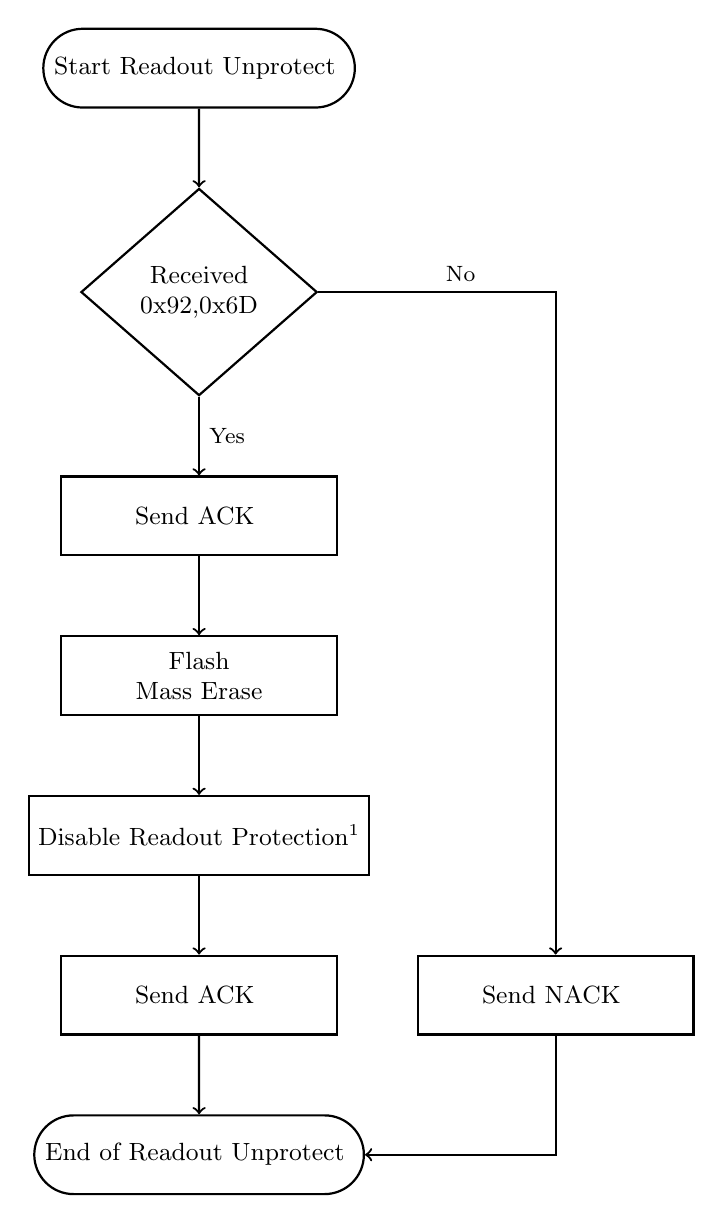
\begin{tikzpicture}[font=\small,thick]
 
\node[draw,
    rounded rectangle,
    minimum width=3.5cm,
    minimum height=1cm,
    align=center
] (block1) { Start Readout Unprotect };

\node[draw,
    diamond,
    below=of block1,
    minimum width=3cm,
    minimum height=2cm,
    align=center
] (block2) { Received\\0x92,0x6D };

\node[draw,
    below=of block2,
    minimum width=3.5cm,
    minimum height=1cm,
    align=center
] (block3Y) { Send ACK };

\node[draw,
    below=of block3Y,
    minimum width=3.5cm,
    minimum height=1cm,
    align=center
] (block4) { Flash\\Mass Erase };

\node[draw,
    below=of block4,
    minimum width=3.5cm,
    minimum height=1cm,
    align=center
] (block5) { Disable Readout Protection\footnotemark };

\node[draw,
    below=of block5,
    minimum width=3.5cm,
    minimum height=1cm,
    align=center
] (block6) { Send ACK };

\node[draw,
    right=of block6,
    minimum width=3.5cm,
    minimum height=1cm,
    align=center
] (block3N) { Send NACK };
 
\node[draw,
    rounded rectangle,
    below=of block6,
    minimum width=3.5cm,
    minimum height=1cm,
    align=center
] (block7) { End of Readout Unprotect };

\draw[->] (block1) -- (block2);

\draw[->] (block2) -- (block3Y) node [pos=0.5,right,font=\footnotesize] { Yes };
\draw[->] (block2) -| (block3N) node [pos=0.3,above,font=\footnotesize] { No };

\draw[->] (block3Y) -- (block4);
\draw[->] (block4) -- (block5);
\draw[->] (block5) -- (block6);
\draw[->] (block6) -- (block7);

\draw[->] (block3N) |- (block7);

\end{tikzpicture}}}
\footnotetext{readout protection is disabled after flash Mass Erase is sucesfully finished}

  
% ------------------------------------------------------------
% ------------------------------------------------------------
  
% END of the KETCube appNote Content

% ------------------------------------------------------------
% ------------------------------------------------------------



% ------------------------------------------------------------
% ------------------------------------------------------------
  
% Insert the common KETCube appNote Tail

% ------------------------------------------------------------
% ------------------------------------------------------------

% ------------------------------------------------------------
% ------------------------------------------------------------
  
% END of the KETCube appNote Content

% ------------------------------------------------------------
% ------------------------------------------------------------


\clearpage
\bibliographystyle{IEEEtran}
\bibliography{IEEEabrv,resources/sources}

%
% Include this license into all KETCube-related documentation
%
%

\clearpage

~

\vfill

\section*{Important Notice}

\subsection*{Copyright}
\copyright ~2018 University of West Bohemia in Pilsen\\
All rights reserved.

\subsection*{Developed by}
The SmartCAMPUS Team\\
Department of Technologies and Measurement\\
Faculty of Electrical Engineering\\
www.smartcampus.cz/en $\mid$ www.zcu.cz/en

\subsection*{License\footnotemark}
\footnotetext{{\it University of Illinois/NCSA Open Source License} (\url{https://opensource.org/licenses/NCSA}) -- similar to {\it Modified BSD License}}

Permission is hereby granted, free of charge, to any person obtaining a copy of this software and associated documentation files (the “Software”), to deal with the Software without restriction, including without limitation the rights to use, copy, modify, merge, publish, distribute, sublicense, and/or sell copies of the Software, and to permit persons to whom the Software is furnished to do so, subject to the following conditions:

\begin{itemize}
    \item[--] Redistributions of source code must retain the above copyright notice, this list of conditions and the following disclaimers.
    \item[--] Redistributions in binary form must reproduce the above copyright notice, this list of conditions and the following disclaimers in the documentation and/or other materials provided with the distribution.
    \item[--] Neither the names of The SmartCAMPUS Team, Department of Technologies and Measurement and Faculty of Electrical Engineering University of West Bohemia in Pilsen, nor the names of its contributors may be used to endorse or promote products derived from this Software without specific prior written permission. 
\end{itemize}
THE SOFTWARE IS PROVIDED “AS IS”, WITHOUT WARRANTY OF ANY KIND, EXPRESS OR IMPLIED, INCLUDING BUT NOT LIMITED TO THE WARRANTIES OF MERCHANTABILITY, FITNESS FOR A PARTICULAR PURPOSE AND NONINFRINGEMENT. IN NO EVENT SHALL THE CONTRIBUTORS OR COPYRIGHT HOLDERS BE LIABLE FOR ANY CLAIM, DAMAGES OR OTHER LIABILITY, WHETHER IN AN ACTION OF CONTRACT, TORT OR OTHERWISE, ARISING FROM, OUT OF OR IN CONNECTION WITH THE SOFTWARE OR THE USE OR OTHER DEALINGS WITH THE SOFTWARE. 

\end{document}


\end{document}


